\documentclass[12pt]{article}
\usepackage{graphicx} % Required for inserting images
\usepackage[margin=0.8in]{geometry}
\usepackage{multicol} % Include the multicol package
\usepackage{titlesec}
\usepackage{array}
\usepackage{multirow}
\usepackage{tabularray}
\usepackage{subcaption} % For subfigures
% \renewenvironment{abstract}

\usepackage[table]{xcolor} % Include xcolor package for defining colors
\usepackage{colortbl} % Include colortbl package for coloring table cells

\usepackage[font=footnotesize,labelfont=bf]{caption}

\titleformat{\paragraph}
{\normalfont\normalsize\bfseries}{\theparagraph}{1em}{}
\titlespacing*{\paragraph}
{0pt}{3.25ex plus 1ex minus .2ex}{1.5ex plus .2ex}

\title{ A Project Report\\ on \\ Exploring Generative Models (Variational Autoencoders) for Audio Generation\\[3.5cm]}

\author{\textbf{By}\\ Rabin Nepal (U00901360)\\ Sravan Kumar Dumpeti (U00905167) \\Department of Electrical and Computer Engineering\\[2cm]}

\date{\textbf{Submitted to} \\ Salim Sazzed, Ph.D \\ [COMP 6741 Intro to Neural Networks] \\ Department of Computer Science \\[2.5cm] UNIVERSITY OF MEMPHIS \\ MEMPHIS, TN, USA \\[2cm] \today\\}

\begin{document}

\begin{titlepage}
    \maketitle
\end{titlepage}


\begin{abstract}
\textit{This project explores the application of Variational Autoencoders (VAEs) in the domain of audio generation, specifically focusing on generating spoken digits. The study employs VAE architectures with Multilayer Perceptron (MLP) and Convolutional Neural Network (CNN) layers for encoding and decoding audio data represented in Short-Time Fourier Transform (STFT) features. A detailed analysis of the trained VAE models is conducted, investigating various training epochs, regularization techniques, and model architectures. The performance of each model variant is evaluated based on training time, loss metrics, and latent space representations. The outcomes provide insights into the efficacy of VAEs for generating high-fidelity audio samples and their ability to learn distinctive representations for spoken digits.
}

\textbf{Keywords:} Generative AI, Audio Synthesis, Variational AutoEncoders, STFT
\end{abstract}

\section{Introduction}
Speech is a unique trait inherent to humans, allowing us to convey thoughts and ideas through vocal sounds. It serves as the most natural method of communication among humans. And even in the area of human-computer interaction, attempts have been made to integrate speech. However, the main issue within this implementation is that all the verbal replies we get from computers, intelligent systems, or artificial intelligence systems still need to be pre-recorded, and the computers themselves do not actually generate speech data. Hence, there is a need to generate speech data that works without the restrictions possessed by the prerecorded audio data.

\subsection{Problem Statement}
The field of Artificial Intelligence (AI) has advanced to a stage where we can now reconstruct or generate many forms of data like images, videos, text, and even complete entire sentences using AI and more specifically generative AI models. Most of the research work in generative models, however, has been on the synthesis/generation of textual data, which is not as natural a form of communication as speech data. The textual data format has also limited the access of the technology to people who have the ability to read and write.

This project will explore the usage of Generative models on audio data to shed more light on the potential usage of such models to generate speech, which is a more inherent form of communication to humans. This project's scope is to explore the use of generative AI models, specifically the VAE (Variational AutoEncoders) model to see how well these models work on audio generation tasks. Through this exploration, the project aims to contribute to the broader understanding of variational autoencoders and their role in audio generation.


\subsection{Literature Review}
The field of artificial intelligence was predominantly used in the prediction or inference task using the vast amount of data available. The idea that AI can actually be used to generate something new was first introduced by Geoffery Hinton and his team in their 2006 paper \cite{Hinton2006Fast}. After the introduction of GANs (Generative Adversarial Networks) in 2014 by Ian Goodfellow, a major leap in the domain of generative AI happened leading to major contributions to the field \cite{Goodfellow2014Generative}. Deep learning frameworks were later distinguished into two main domains: a) Generative Frameworks and b) Discriminate Frameworks.
\begin{enumerate}
    \item \textbf{Discriminative AI: }Discriminative AI deals with models that separate given data instances into different classes by learning the differences within the dataset. Image classification through Convolution Neural Is an example of discriminative AI.
    \item \textbf{Generative AI: }Generative AI, instead of learning the differences in data, tries to learn the actual distribution of data and tries to generate new data samples using the learned distribution of data. 
\end{enumerate}

Many generative architectures have been developed after its introduction but the two most famous are the VAE (Variational AutoEncoders), which this project aims to utilize for the generation of audio samples,  and GANs (Generative Adversarial Networks).

Audio data has been primarily used as an input to the machine learning models, mostly made famous by Google’s speech recognition engine. Traditional methods for audio synthesis often rely on physical modeling or rule-based approaches, which can be computationally expensive and limited in their generative/synthesis potential. Generative models, on the other hand, offer a data-driven approach that allows for more flexible and realistic audio generation. There also have been works in the Speech Synthesis task from the past but mostly focused on text-to-speech synthesis to convert written text into spoken words, trying to mimic the human form of speech. Generative models have revolutionized the field of audio synthesis and sound manipulation in recent years. These models are capable of learning complex statistical relationships within audio data and subsequently generating novel audio samples that closely resemble real-world examples. \cite{Natsiou2021Audio}

From our review of the existing literature, we have classified the audio generation task into three main domains: a) Music Generation b) Speech Synthesis c) Sound Effects Generation. This project will focus on the speech synthesis domain and try to generate new discrete samples of human speech, namely spoken digits, in this case. A work in this domain by \cite{Becker2018Interpreting} explores the use of an end-to-end generative model with a hierarchical architecture combining autoregressive multilayer perceptrons and recurrent neural networks, capturing the long-range dependencies in the audio.

More complex models like WaveNet by DeepMind \cite{Oord2016WaveNet}, utilize dilated causal convolutional architectures with very large receptive fields to capture long-range temporal dependencies that generate even more natural-sounding audio achieving state-of-the-art performance. WaveNet showed excellent performance in all three domains of audio generation mentioned above. This model, however, is computationally expensive making it harder to implement in real-time generation tasks.

Microsoft has also designed a robust speech generation AI framework called FastSpeech with MFCC (Mel-Frequency Cepstral Coefficients) and a feed-forward-based Transformer model to generate natural speech. As its name implies, it is a faster generative model that achieves 270 times the speed in MFCC generation and 38 times faster on entire speech synthesis compared to existing models at that time.\cite{Ren2019FastSpeech}

Another work by Chris Donaheu et al from UC San Diego \cite{Donahue2018Adversarial} proposed their model WaveGAN to synthesize raw waveform audio itself. The models produced excellent results even when trained on a small dataset, and utilized an existing GAN architecture like DCGAN, primarily used in the image synthesis domain, with some modifications to implement them to generate audio samples. Due to its parallel nature, the model also showed computational efficiency and could generate hours of raw audio in seconds. All these works utilized complex models and huge datasets to achieve speech generation. This project on the contrary explores the potential of a simple VAE model for this task.

\section{Dataset}
This project will utilize the audio version of the MNIST dataset made available by, a rich resource for exploring spoken digit recognition task. The AudioMNIST dataset offers a rich and diverse resource for exploring spoken digit recognition research. Its large size, speaker diversity, and high-quality audio format provide a solid foundation for developing robust and generalizable models for recognizing spoken digits.

\begin{figure}[!h]
    \centering
    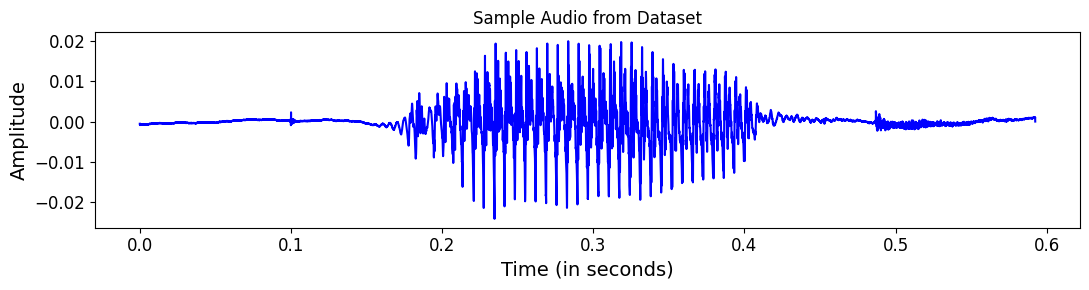
\includegraphics[width=0.75\linewidth]{figures/sample audio.png}
    \caption{Audio Signal (Waveform) for Digit 9}
    \label{fig:enter-label}
\end{figure}

Here's a detailed analysis of the dataset:

\subsection{Data Composition and Size}
The dataset contains audio recordings of all digits (0-9) spoken by 60 different speakers, totaling 30,000 samples (making it 3000 samples for each digit). This provides a substantial amount of data for training and evaluating spoken digit recognition models. The total duration of the recordings is 9.5 hours, offering a diverse range of speech patterns and pronunciations. This diversity can help train a generative model that encompasses variations in speech characteristics.

\begin{figure}[!h]
    \centering
    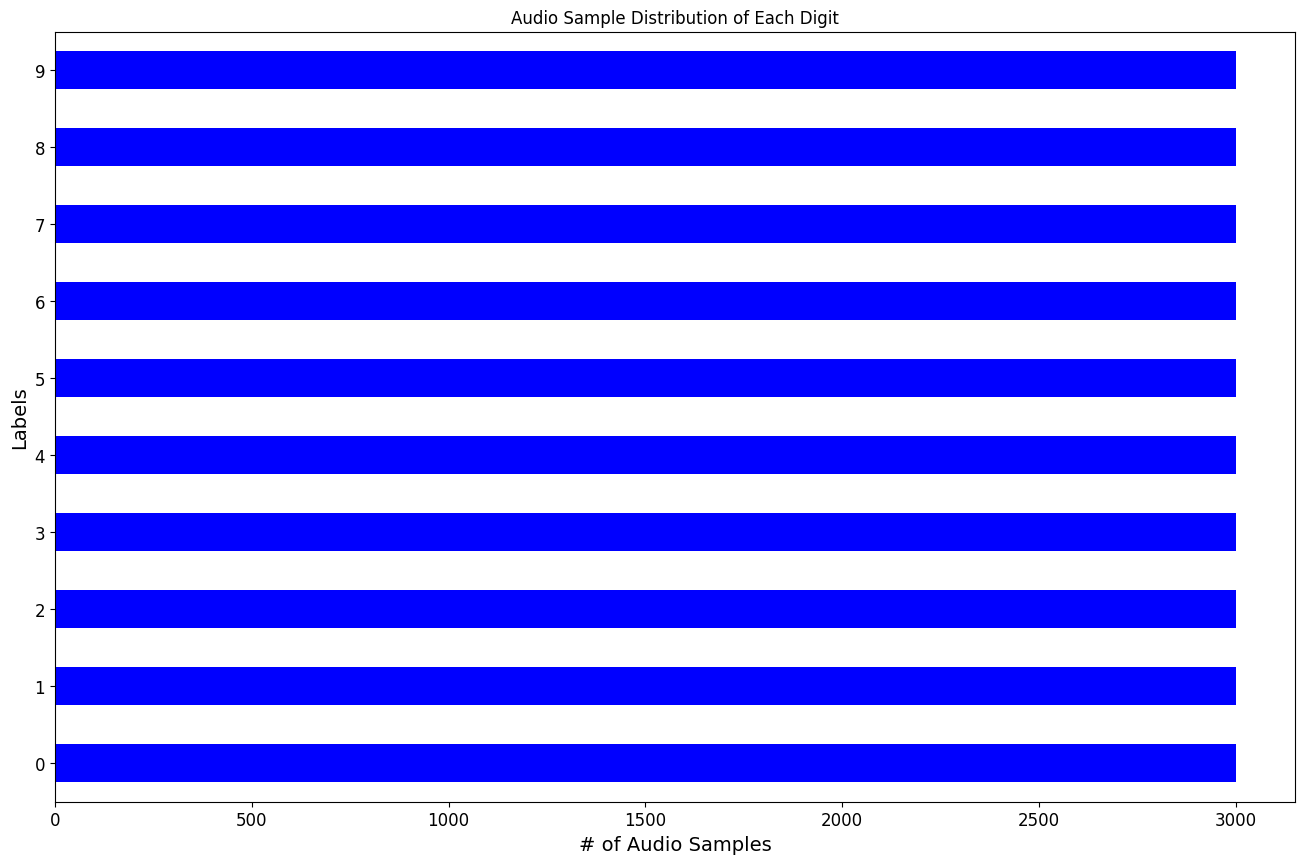
\includegraphics[width=0.6\linewidth]{figures/sample distribution.png}
    \caption{Distribution of Audio Samples for each Digit in the Dataset}
    \label{fig:enter-label}
\end{figure}



\subsection{Speaker Diversity}
The dataset includes recordings from speakers with a wide range of accents, encompassing both native and non-native English speakers. This diversity is crucial for developing models that generalize well to different pronunciations and speech patterns.

\begin{figure}[h!]
    \centering
    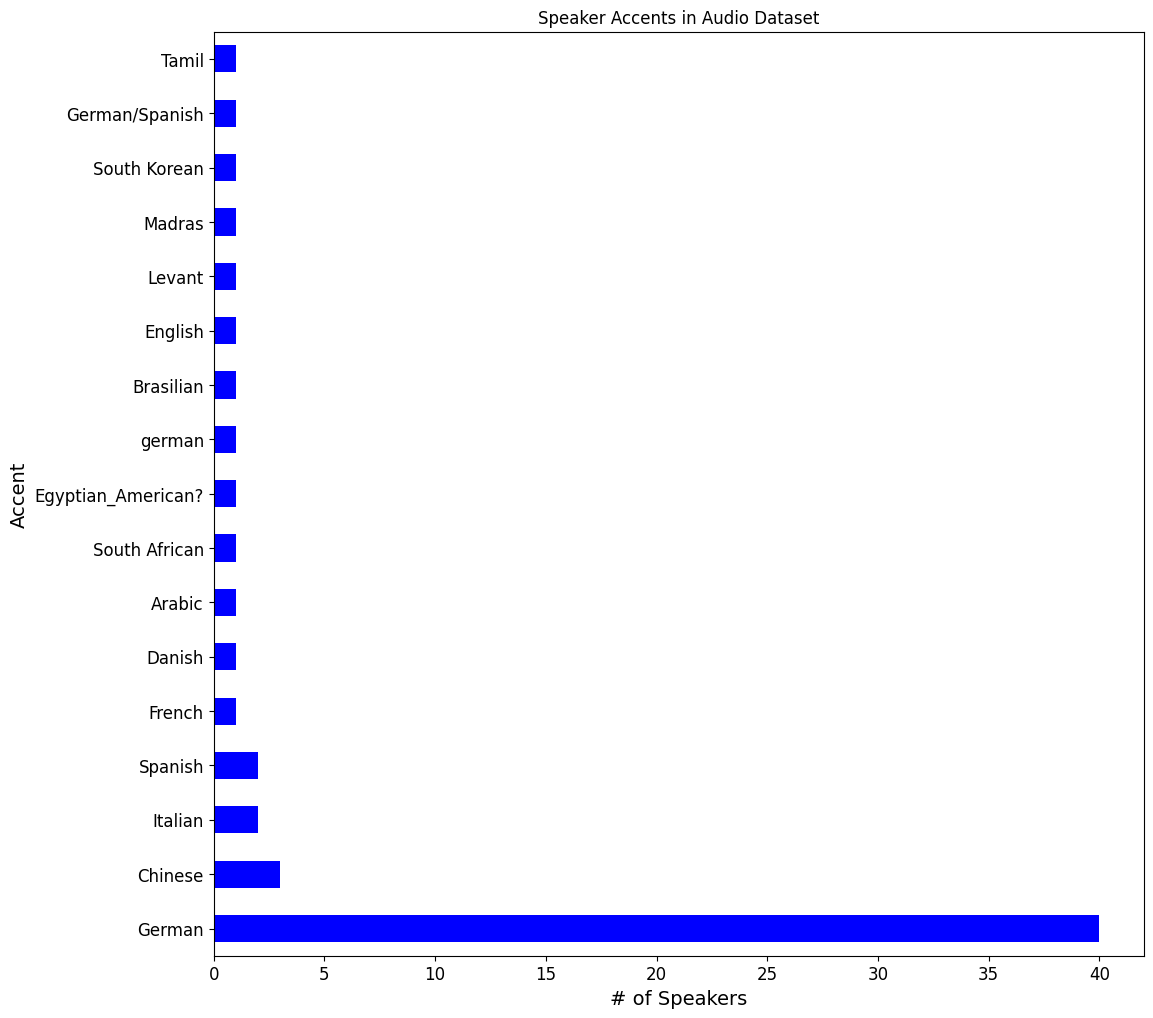
\includegraphics[width=0.6\linewidth]{figures/speaker diversity.png}
    \caption{Distribution of Speaker's Accent in the Dataset}
    \label{fig:enter-label}
\end{figure}

\subsection{Audio Specifications}
Each audio sample is recorded in single-channel format with 16-bit resolution and a sampling rate of 48 kHz. This high-quality format preserves the important details of the spoken digits, allowing for accurate analysis and modeling.

\subsection{Data Challenges and Considerations}
\begin{itemize}
    \item The diversity of accents and speaker characteristics, while beneficial, also presents challenges for model robustness. Specific training strategies or feature engineering might be necessary to address speaker variability.
    \item The single-channel format of the audio data might limit the exploration of advanced techniques that utilize spatial information for improved recognition.
    \item The dataset size, while substantial, may still be considered moderate for training complex deep-learning models. Especially in our case where we are trying to build a generative model to learn all possible representations for each of the digits in the dataset.  Having 3000 samples (and even fewer after data processing) per digit could be a potential issue for the generative task.
\end{itemize}





\section{Methodology}

\begin{figure}[h!]
    \centering
    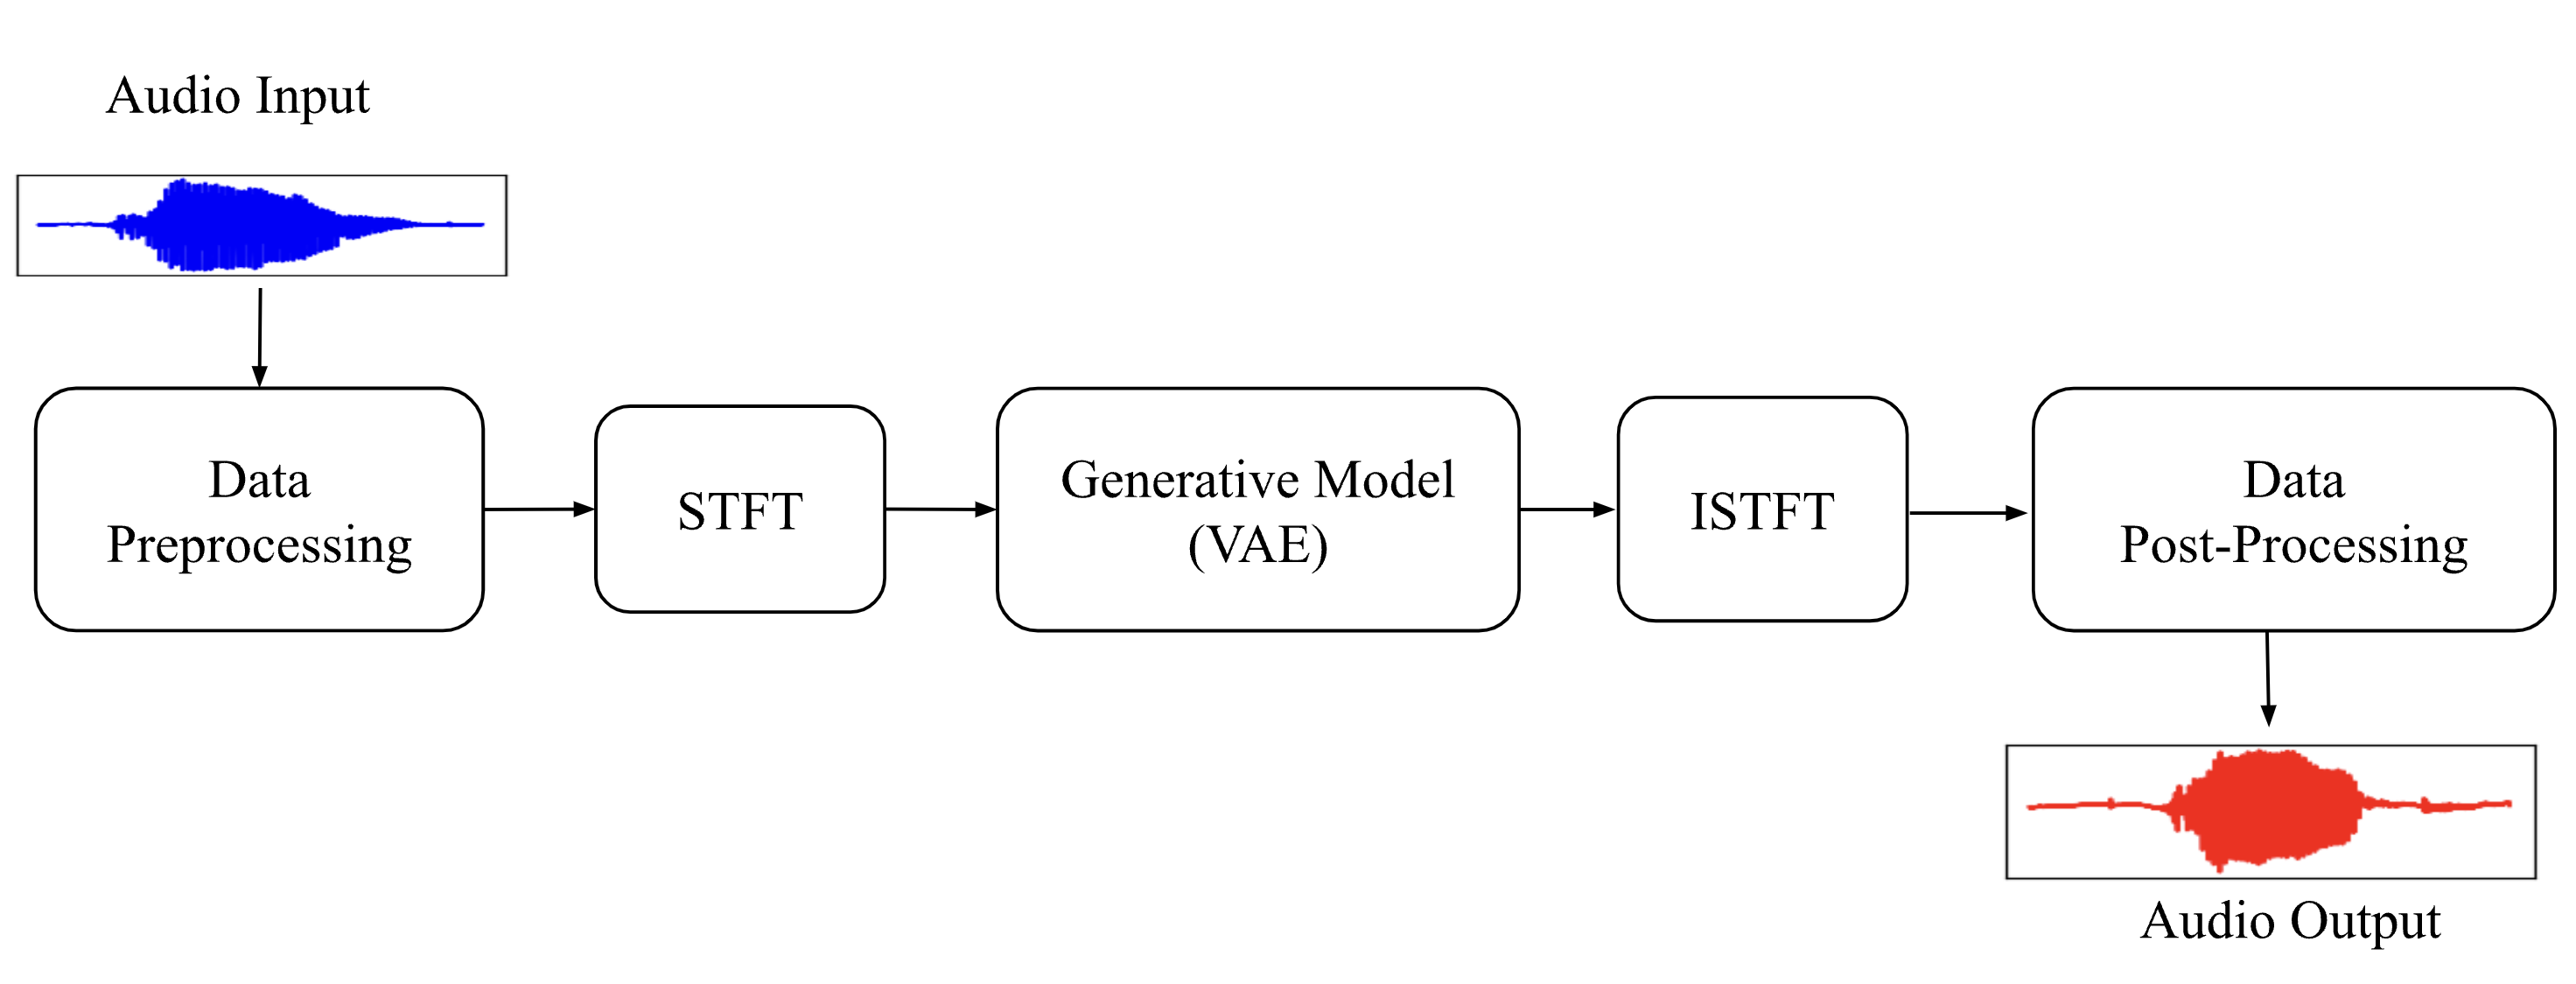
\includegraphics[width=0.9\linewidth]{figures/method.png}
    \caption{Block Diagram of the Proposed Audio Generation System}
    \label{fig:enter-label}
\end{figure}


Fig. 1 depicts the proposed system for the audio generation task. The input to the system is an audio sample of spoken digits (explained further below). The steps include data preprocessing, feature extraction using STFT (Short Time Fourier Transform), and feeding into a generative model (Variational Autoencoder in this case), which gives a newly generated STFT for generated audio data. The ISTFT (Inverse Short Time Fourier Transform) block reconverts the signal back to an audio signal. This signal is then sent to a data post-processing block which does the necessary post-processing. Finally, a properly generated audio can be observed from the system. The steps have been discussed further in detail:

\subsection{Data Preprocessing}
Audio data from the dataset can include recordings with different lengths, different amplitudes, and silences or there could be data samples with faulty recordings. The data preprocessing step eliminates this inconsistency in data samples. The preprocessing done in the dataset has been described below:

\subsubsection{Downsampling Audio Signal}
The first processing applied to the audio signal is downsampled it to a lower frequency. The recorded audio signal is sampled at 48KHz which means there are 48000 samples per second. Such a large number of samples per second decreases the computational efficiency and hinders in feature extraction and model training. Since an audio signal can retain its fidelity, the audio signal is resampled at 22.05KHz without losing any information during the downsampling process.

\subsubsection{Filtering Outliers}
The dataset also had exceptionally long and exceptionally short audio samples in them. These outliers were removed with reference to the 1st and 99th percentile of the length of the samples, where any values beyond these were removed.

\begin{figure}[!h]
    \centering
    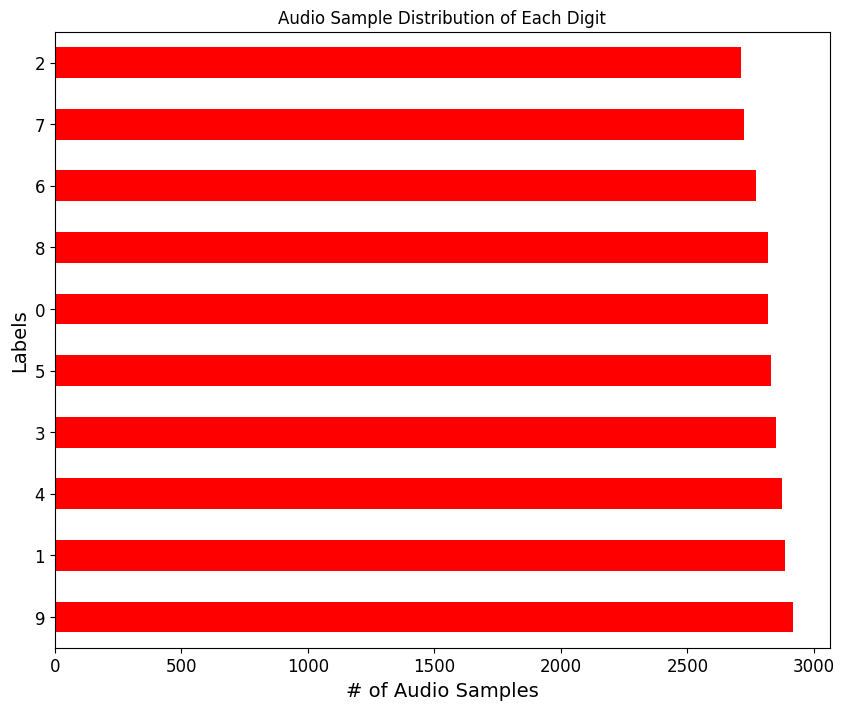
\includegraphics[width=0.5\linewidth]{figures/audio after filtering data.png}
    \caption{Sample Distribution After Removing Outliers: In contrast to the \textbf{figure 2},  we can see a decrease in the number of samples in some digits.}
    \label{fig:enter-label}
\end{figure}

\subsubsection{Audio Length Normalization}
The next step in audio data pre-processing is the normalization of audio samples. Given the variability in speaking rates among different speakers, identical digits might exhibit diverse durations (measured in seconds). The normalization process for audio length involves manipulating the downsampled audio signal. Specifically, audio segments exceeding a duration of 0.87 seconds are trimmed, while those with durations less than 0.8 seconds are augmented by padding the audio signal with zeros. The selection of 0.87 seconds as the threshold stems from an analysis of the distribution of audio lengths, where this duration encompasses nearly all instances (approximately 97th percentile) of the audio samples.

\begin{table}[!h]
\centering
\caption{Percentile of Audio Lengths}
\label{tab:my_table}
\begin{tabular}{l|l|l}
\textbf{Percentile} &\textbf{ Audio Length(in \# of samples)} & \textbf{Audio Length(in seconds)} \\ \hline
1\textsuperscript{st} & 9391.94 & 0.426 \\
3\textsuperscript{rd} & 10150.0 & 0.460 \\
10\textsuperscript{th} & 11168.0 & 0.507 \\
50\textsuperscript{th} & 13936.0 & 0.632 \\
95\textsuperscript{th} & 18502.0 & 0.839 \\
\textbf{97}\textbf{\textsuperscript{th}} & \textbf{19185.03} & \textbf{0.870} \\
99\textsuperscript{th} & 20485.01 & 0.920 \\

\end{tabular}
\end{table}

% \begin{figure}[htbp]
%     \centering
%     \begin{subfigure}[b]{0.45\textwidth}
%         \centering
%         \includegraphics[width=\textwidth]{figures/sample_before_normalization.png}
%         \caption{Histogram of Audio Lengths before Length Normalization}
%         \label{fig:left_figure}
%     \end{subfigure}
%     \hfill
%     \begin{subfigure}[b]{0.45\textwidth}
%         \centering
%         \includegraphics[width=\textwidth]{sample_after_normalization.png}
%         \caption{Histogram of Audio Lengths after Length Normalization}
%         \label{fig:right_figure}
%     \end{subfigure}
%     \caption{Main Caption}
%     \label{fig:main_figure}
% \end{figure}


\begin{figure}[htbp]
    \centering
    \begin{minipage}[b]{0.45\linewidth}
        \centering
        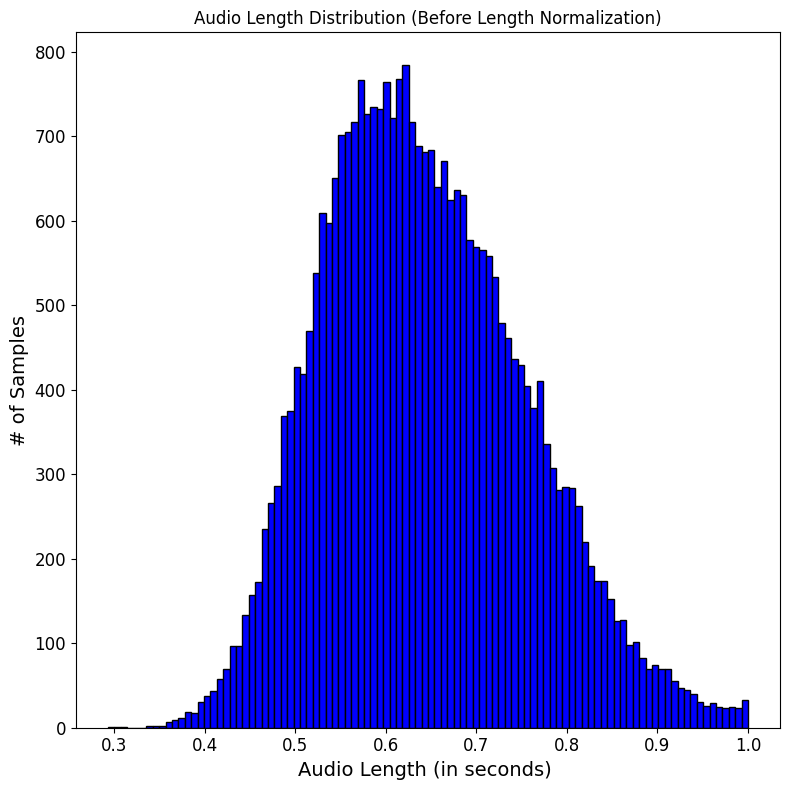
\includegraphics[width=\linewidth]{figures/sample before normalization.png}
        \caption{Histogram of Audio Lengths before Length Normalization}
        \label{fig:high_freedom}
    \end{minipage}
    \hfill
    \begin{minipage}[b]{0.45\linewidth}
        \centering
        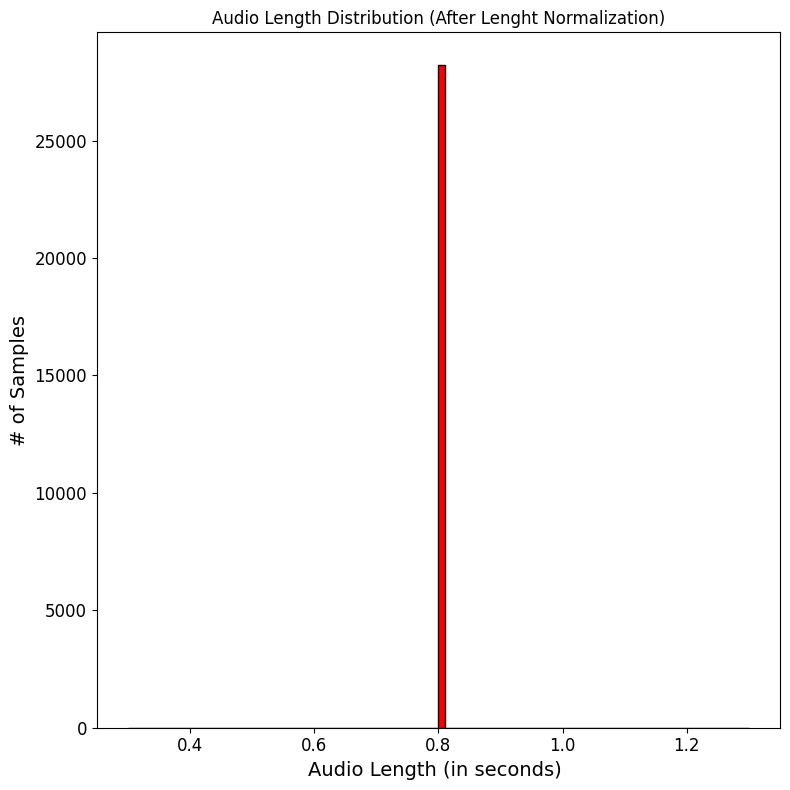
\includegraphics[width=\linewidth]{figures/sample after normalization.png}
        \caption{Histogram of Audio Lengths after Length Normalization}
        \label{fig:least_freedom}
    \end{minipage}
\end{figure}






\subsubsection{Amplitude to Log Scale}
Following length normalization, the audio signal is prepared for spectral feature extraction, essential for input into the generation model. The Short-Time Fourier Transform (STFT) generates a spectrogram, portraying time on the x-axis, frequency on the y-axis, and intensity representing the magnitude or power of frequencies at each instance. The amplitude of STFT is transformed to a log scale in this data preprocessing step. Transforming the amplitude values of the STFT into a log scale helps compress the dynamic range, enhances visualization, aligns with auditory perception, aids in noise reduction, and can contribute to a more stable and effective model.

\subsubsection{Min-Max Normalization of STFT}
The subsequent step in data preprocessing involves applying min-max normalization. The varying log magnitudes present in the STFT output can affect the stability of the model throughout training, thereby influencing the speed of convergence and the dynamics of training. To address this, the STFT output undergoes min-max normalization. This normalization technique aims to secure a stable training process while enhancing both convergence and dynamics.

\subsubsection{Train-Validation-Test Split}
Finally, the dataset was split into training, validation, and testing data. The purpose was to allocate specific portions for training the model, validate its performance during training, and independently assess its accuracy and generalization on unseen data.

Initially, the entire dataset was partitioned using a 9:1 ratio, allocating 90\% to the training set and 10\% to the test set. Within the 90\% allocated for training, a subsequent 9:1 ratio split further divided the data into training and validation sets.

\begin{itemize}
    \item \# of samples in Training Data: \textbf{22840}
    \item \# of samples in Validation Data: \textbf{2538}
    \item \# of samples in Testing Data: \textbf{2820}
\end{itemize}


\begin{figure}[!h]
    \centering
    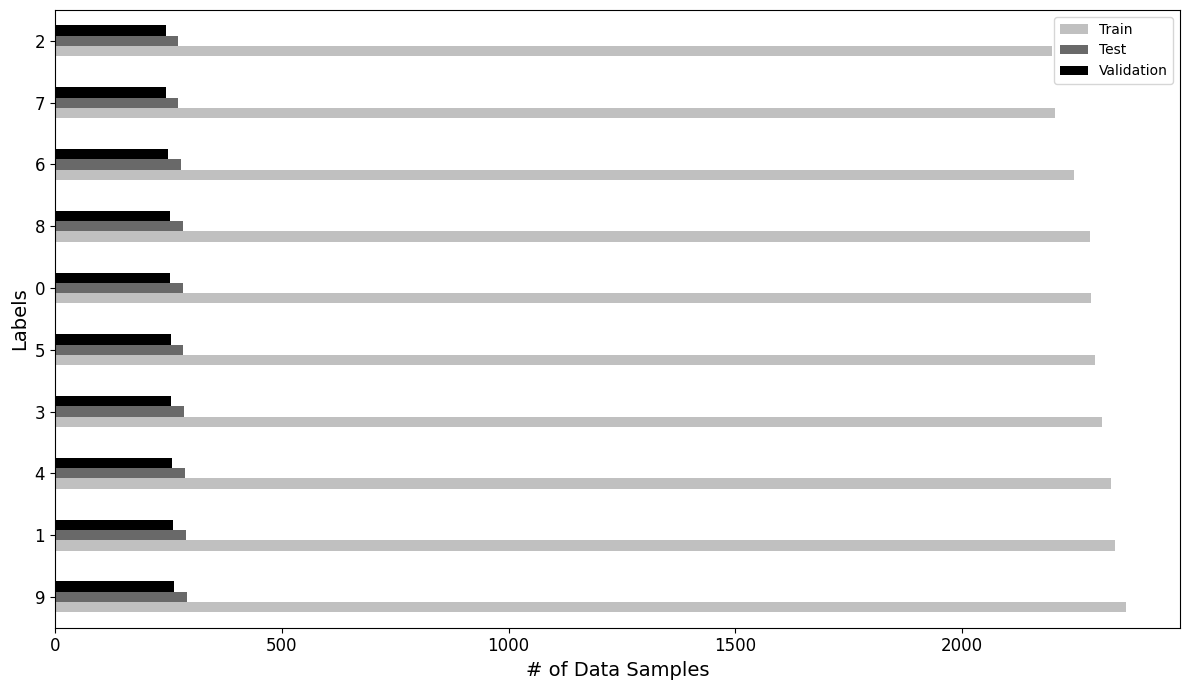
\includegraphics[width=0.75\linewidth]{figures/train_test.png}
    \caption{Sample Distribution in Train, Validation and Test Set}
    \label{fig:enter-label}
\end{figure}


\subsection{STFT}
STFT is a way of observing the frequency and phase content of a signal over time. It provides a localized time-frequency representation of the signal that allows us to observe the changes in frequency over time more accurately. This is crucial for understanding the differences among the different audio digits in the dataset. The output of an STFT is the amplitude of the audio signal represented in time and frequency. The window length of 512 samples was used and the said window was applied at every 256 samples (stride of the STFT). We also explored the use of MFCC for this project. MFCC has proven to be the best feature extraction method for audio recognition tasks and we were hopeful it would be excellent for audio generation too. However, upon further research, we found out that obtaining an audio signal from MFCC is complex and does retain as high fidelity as inverse STFT. So, we decided to use STFT for this project.

\begin{figure}[htbp]
    \centering
    \begin{minipage}[b]{0.45\linewidth}
        \centering
        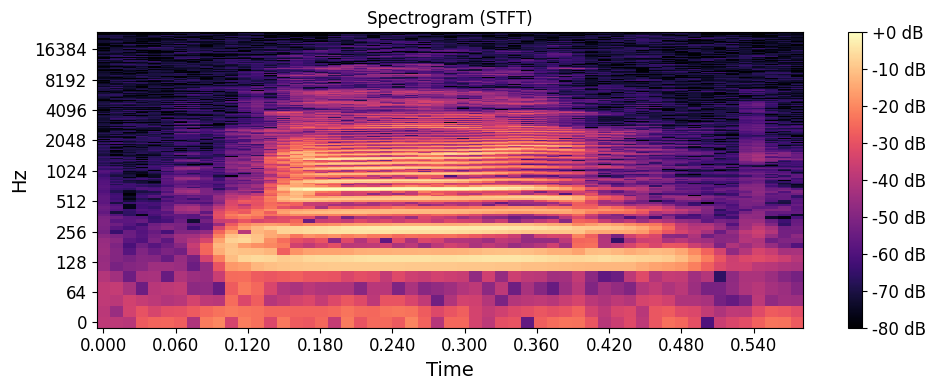
\includegraphics[width=\linewidth]{figures/spectogram.png}
        \caption{Spectogram of Input Audio before Length Normalization}
        \label{fig:high_freedom}
    \end{minipage}
    \hfill
    \begin{minipage}[b]{0.4\linewidth}
        \centering
        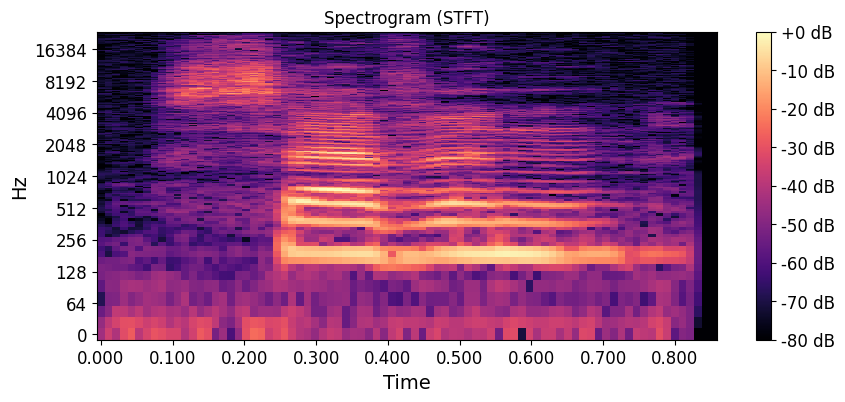
\includegraphics[width=\linewidth]{figures/spectogram after normalization.png}
        \caption{Spectogram of Input Audio  after Length Normalization}
        \label{fig:least_freedom}
    \end{minipage}
\end{figure}





\subsection{Generative Model - Variational AutoEncoder (VAEs)}
Variational Autoencoder is the generative model proposed for this study. This model is an unsupervised learning method that can learn the distribution of the data to generate new data. VAE architecture is composed of an encoder and decoder that is trained to minimize the reconstruction error between the encoded-decoded data and initial data. The encoder of VAE is responsible for mapping the dataset into a latent representation, which is a joint probability distribution of the samples. A random sample data is sampled from the latent representation (joint probability distribution) by the decoder. This sampled data is a reconstruction of data from the latent space. The reconstruction error is calculated using the input and reconstructed data, and the model is trained to minimize the reconstruction error. \cite{Goodfellow2016Deep}

\begin{figure}[!h]
    \centering
    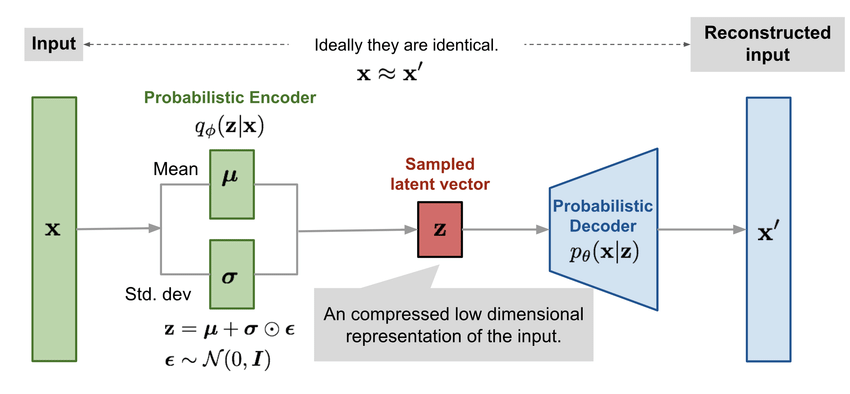
\includegraphics[width=0.75\linewidth]{figures/vae-arch.jpg}
    \caption{Architecture of Variational AutoEncoders \cite{Weng2018From}}
    \label{fig:enter-label}
\end{figure}

The above figure shows a generic architecture for variational autoencoders. VAEs are similar to autoencoders in functionality except for the fact that VAEs maps their input to a distribution, unlike autoencoder which maps their input to a fixed vector. Based on functionality, the architecture can be broken down into three main components:

\textbf{A. Encoder Layer}
The Encoder Layer is tasked with converting input data into a latent space representation, encapsulating the probabilistic distribution of latent variables. The encoder function \(q_\phi(z|x)\) maps the input \(x\) to the parameters of a probability distribution in the latent space. It produces the mean (\(\mu\)) and variance (\(\sigma^2\)) of a Gaussian distribution.

\textbf{B. Latent Layer}
It represents the learned latent variables, typically in the form of a probability distribution (e.g., Gaussian distribution) within the latent space. A sampling from this distribution is done to generate new previously unseen samples.

\textbf{C. Decoder Layer}
It reconstructs data samples from the latent space representation back to the original input space, generating outputs that resemble the input data. The decoder function \(p\_\theta(x|z)\) reconstructs the input data \(x\) from the latent variable \(z\). It maps the latent variable \(z\) back to the data space.

In a Variational Autoencoder (VAE), the loss function comprises two terms: the reconstruction loss and the regularization term, commonly represented as the Kullback-Leibler (KL) divergence. The reconstruction loss measures the dissimilarity between the original input and the output reconstructed by the VAE. It represents how well the model can reconstruct the input data. The regularization term encourages the learned latent space distribution to align with a predefined prior distribution (e.g., a standard Gaussian distribution). This regularization aids in shaping the learned distribution toward desired properties. The optimization of the VAE involves maximizing the Evidence Lower Bound (ELBO) during training. Given the intractability of the posterior probability in VAE due to model complexity, maximizing the ELBO serves as an approximation technique through variational inference, enabling effective parameter optimization and approximation of the true posterior distribution. \cite{Foster2023-yo}

\subsubsection{VAE with MLP}
\begin{figure}[!h]
    \centering
    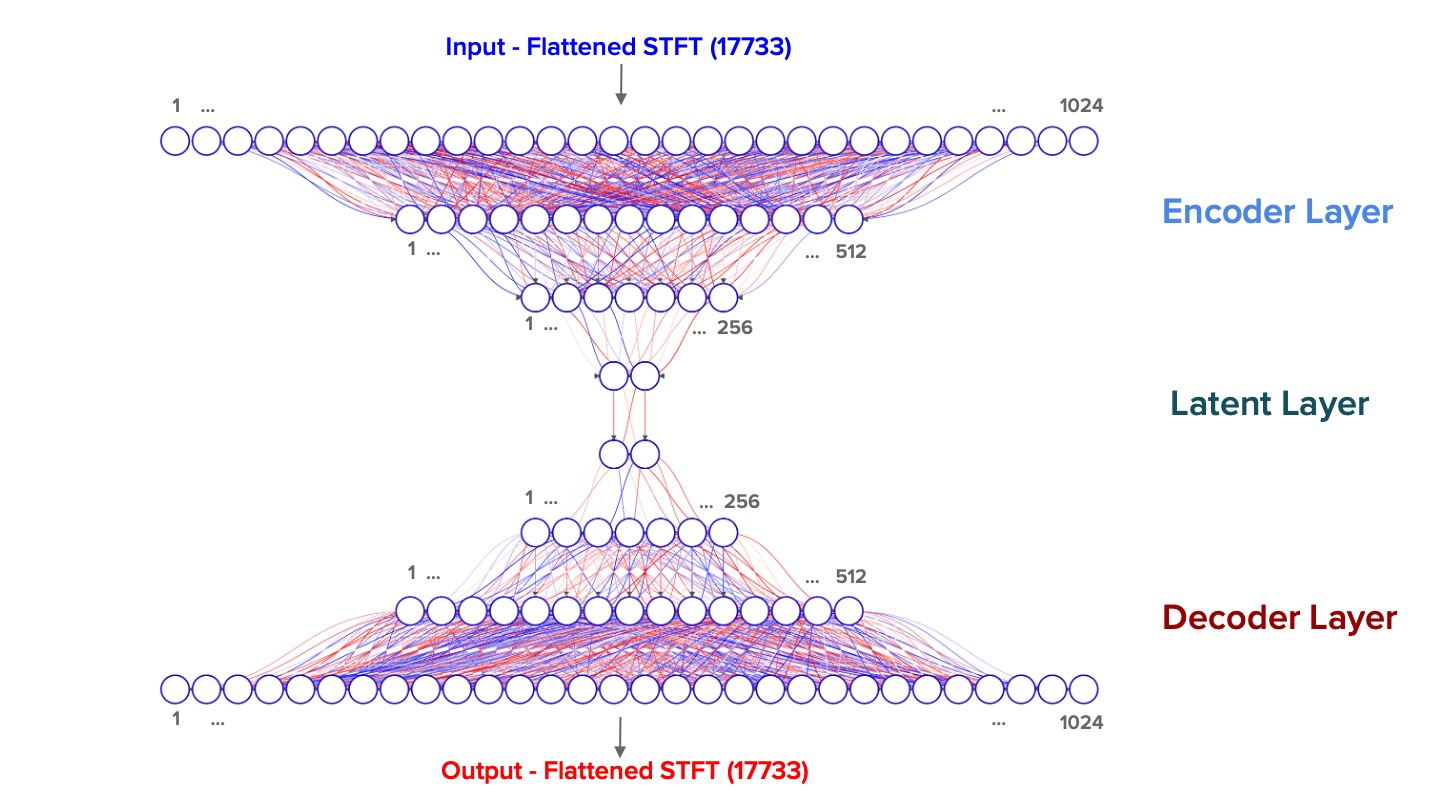
\includegraphics[width=1\linewidth]{figures/VAE-MLP Arch.jpg}
    \caption{Architecture of VAE-MLP (Drawn with \cite{LeNail2019})}
    \label{fig:enter-label}
\end{figure}
The initial model explored for the audio generation task in this project was a deep Variational Autoencoder (VAE) a straightforward VAE employing a multilayer perceptron structure for both encoding and decoding:

\paragraph{Input}
After the data preprocessing step, we are left with two-dimensional STFT features containing the log amplitudes. The input to the model was this STFT flattened to a one-dimensional vector of length 17733.

\paragraph{Encoder Layer}
\begin{itemize}
    \item The encoder consisted of three fully connected layers with decreasing numbers of hidden units to progressively compress the input data into a low-dimensional latent space.
    \item The first layer had 1024 neurons, the second layer had 512 neurons, and the third layer had 256 neurons.
\end{itemize}

\paragraph{Latent Layer}
\begin{itemize}
    \item The dimension of latent space defined in this case was 2 represented by the top pair of neurons in the latent layer as shown in the figure above.
    \item The other pair of neurons in the latent layer represents the sampling layer responsible for sampling new representation from the learned distribution.
\end{itemize}

\paragraph{Decoder Layer}
\begin{itemize}
    \item The sampled representation is then passed onto the decoding layer that mirrors the encoder structure, with three fully connected layers with increasing numbers of neurons to progressively reconstruct the audio data from the latent space.
    \item The first layer had 256 neurons, the second layer had 512 neurons, and the third layer had 1024 neurons.
\end{itemize}

\paragraph{Output}
Finally, the output from the decoder layer produced a generated flattened STFT (Short-Time Fourier Transform) signal of length 17733 (similar to our input), later reshaped to restore its original dimensions.

\subsubsection{VAE with CNN}
\begin{figure}[!h]
    \centering
    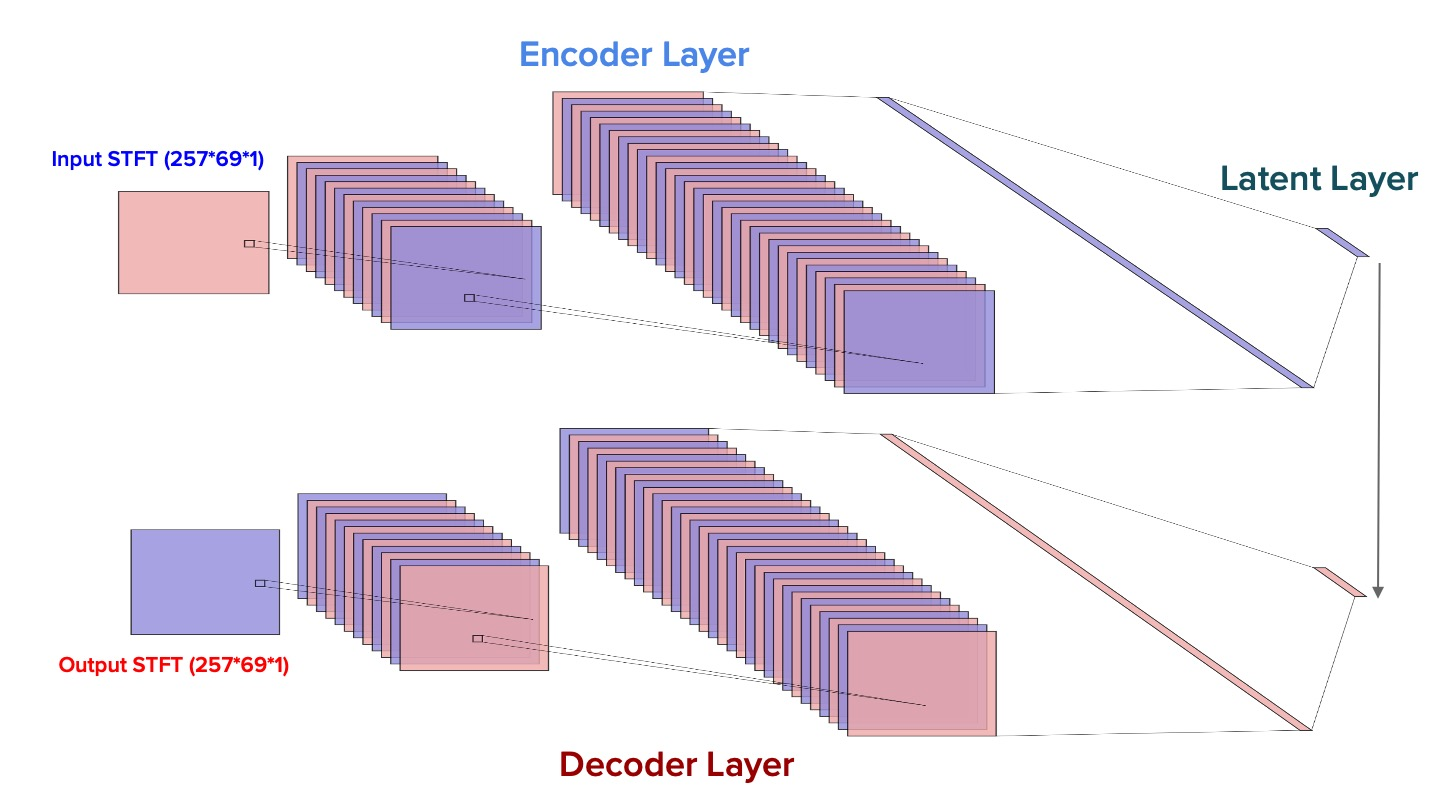
\includegraphics[width=1\linewidth]{figures/VAE-CNN.jpg}
    \caption{Architecture of VAE-CNN (Drawn with \cite{LeNail2019})}
    \label{fig:enter-label}
\end{figure}
The other model explored for audio generation was VAE with Convolutional Neural Network (CNN) as the encoding and decoding layers:

\paragraph{Input}
Unlike VAE with MLP, the input for VAE with CNN required no flattening of the data as the CNN encoder layer can take higher dimensional array input. Therefore, the normalized STFT after data pre-processing was passed to the network as is.

\paragraph{Encoder}
\begin{itemize}
    \item The encoder layer consisted of two convolutional networks and a dense layer at the end
    \item The first convolutional layer used 32 filters with a 3x3 kernel size and employed padding to maintain input-output dimensions.
    \item The second convolutional layer employed 64 filters with a similar 3x3 kernel size and similar padding to the first convolutional network.
    \item The output from the convolutional layers was flattened and subsequently passed through a dense layer containing 256 nodes.
\end{itemize}

\paragraph{Latent Layer}
Following the dense layer, the data was directed to a latent layer consisting of 2 dimensions as represented by the end of the encoding layer in the above figure. Similar to VAE with MLP, sampling was done to sample new data from the learned representation as denoted by the rightmost layer in the decoding layer.

\paragraph{Decoder}
\begin{itemize}
    \item The sampled latent space representation was then used to reconstruct the STFT through the decoding layer.
    \item Initially, a dense layer of 256 neurons (similar to the encoding layer) was used to scale up the low-dimensional latent representation.
    \item The decoding layer then consisted of two convolutional layers similar to the encoder but in reverse order, where
\begin{itemize}
        \item The first convolutional layer consisted of 64 filters of size 3x3 implemented with padding.
        \item The second convolutional layer consisted of 32 filters of size 3x3 implemented with padding.
        \item Finally, the convolved features were resized to the dimension of the input STFT.
\end{itemize}
\end{itemize}

\paragraph{Output}
VAE with CNN model gave an output which itself was the generated STFT for an audio signal.


\subsection{ISTFT}
The ISTFT block of the system is responsible for recovering the original signal from the transformed signal by STFT. The output of the VAE model is a newly generated STFT of MNIST audio data, which needs to be converted back to an audio signal so that the generated output can be heard.

\begin{figure}[!h]
    \centering
    \begin{minipage}[b]{0.45\linewidth}
        \centering
        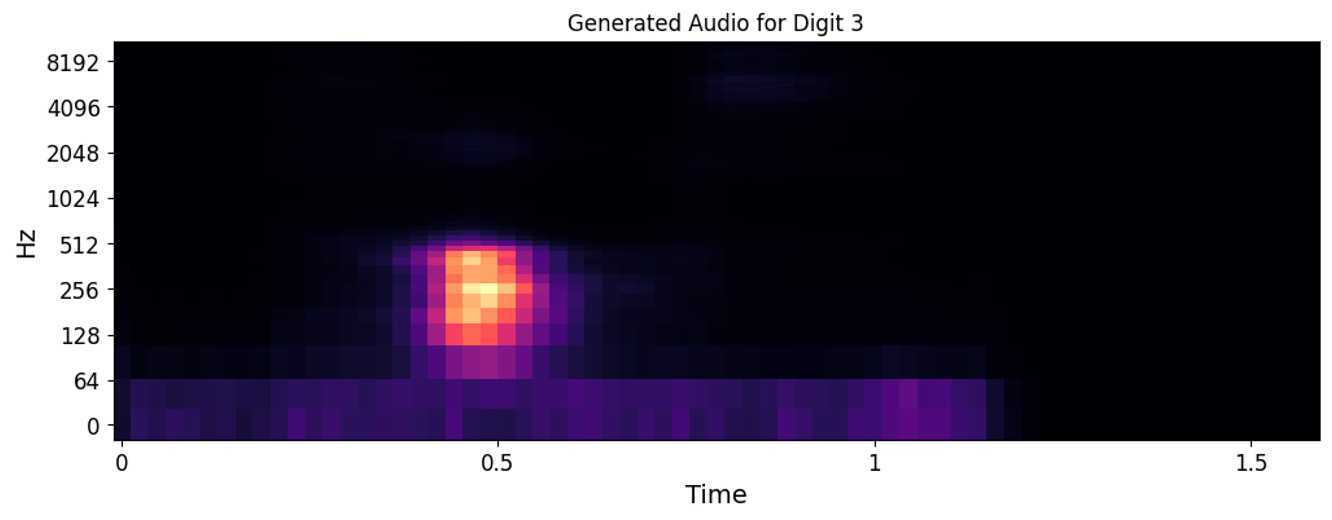
\includegraphics[width=\linewidth]{figures/gen_stft.png}
        \caption{Generated STFT from Generative Model}
        \label{fig:gen_stft}
    \end{minipage}
    \hfill
    \begin{minipage}[b]{0.45\linewidth}
        \centering
        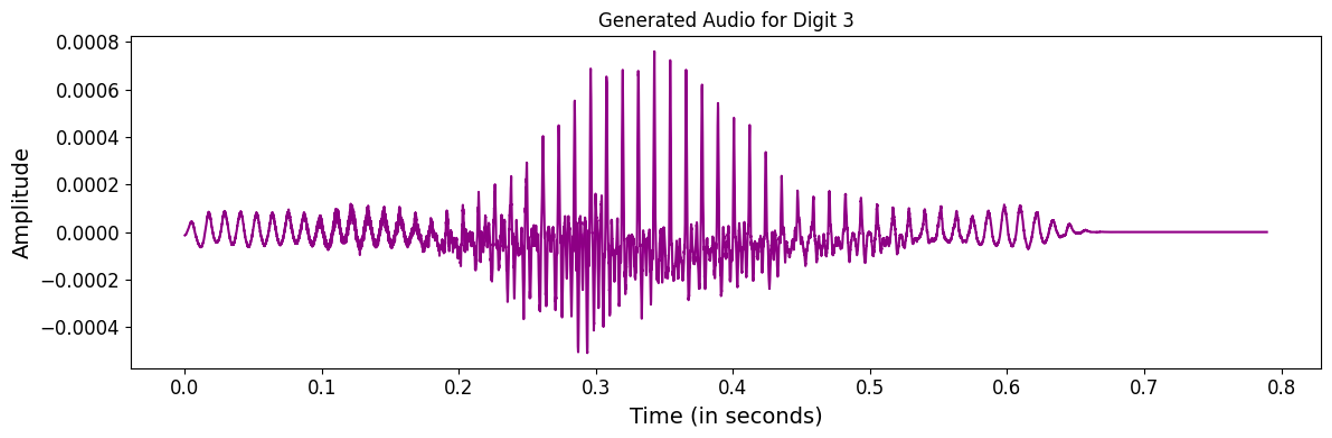
\includegraphics[width=\linewidth]{generated_audio.png}
        \caption{Generated Audio Signal after iSTFT}
        \label{fig:generated_audio}
    \end{minipage}
\end{figure}


\subsection{Data Post-Processing}
Data post-processing is the final stage of the system that is used to transform the generated data from the generative model to a proper format that can be heard. The post-processing happens in two stages:

\subsubsection{Before iSTFT}
Specifically, the generated STFT from the models is first scaled back to proper amplitude using the saved maximum and minimum values during the min-max normalization process. The amplitudes are then converted to a linear scale from a log scale and only then passed to the iSTFT block to convert them back to audio signals.

\subsubsection{After iSTFT}
The audible signal at this stage may not yet be audible due to the low amplitude of audio data the same alterations in frequency domain during the ISTFT process or any other issue that can make the generated audio not audible. This stage of data post-processing aims to eliminate such issues.

\section{Results}
% 

% \subsection{VAE with MLP Models}

% \subsubsection{VAE-MLP (50 Epochs)}
% During the experimentation phase, three variations of the VAE with MLP were trained and evaluated. The architecture defined in section 3.3.1 was used to train the flattened STFT features.

% Initially, a basic VAE-MLP model was trained for 50 epochs, and its training and validation losses were visualized. Observing the loss plot, both the training and validation loss were decreasing and showed no signs of overfitting or underfitting.

% \begin{figure}[htbp]
%     \centering
%     \begin{minipage}[b]{0.45\linewidth}
%         \centering
%         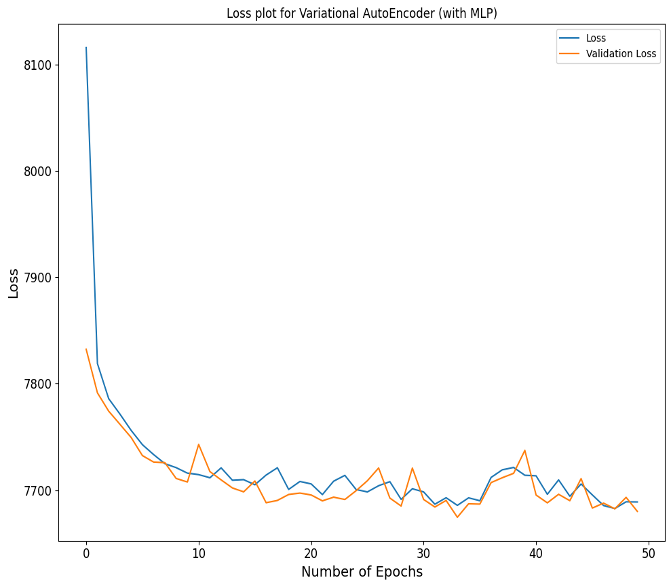
\includegraphics[width=\linewidth]{mlp_vae_50.png}
%         \caption{Loss Curves for VAE-MLP Model trained for 50 epochs}
%         \label{fig:gen_stft}
%     \end{minipage}
%     \hfill
%     \begin{minipage}[b]{0.45\linewidth}
%         \centering
%         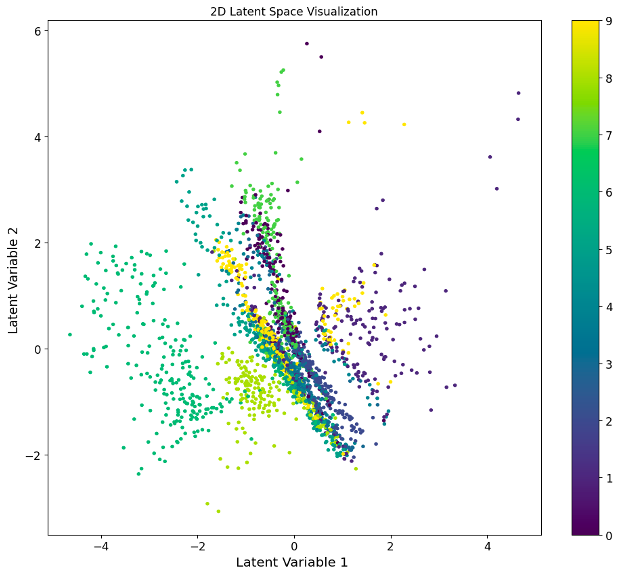
\includegraphics[width=\linewidth]{mlp_vae_lat.png}
%         \caption{Latent Space Visualization on test data for VAE-MLP Model Trained for 50 epochs}
%         \label{fig:generated_audio}
%     \end{minipage}
% \end{figure}

% Since the model showed promise, we decided to observe the learned latent space representation of the model. However, the visualization clearly showed severe overlapping of the learned representations for certain digits (especially for digits 0,1,2,3, and 9), indicating the model has not learned distinctive representations for each of the digits yet. Observing the loss plot again, it was evident that while the model was learning, there remained room for additional improvement since both the losses displayed potential for further decrease (that is the losses were not observed to be saturated) in loss and learning the representations better. We therefore decided to train the model for more epochs.

% \subsubsection{VAE-MLP (100 Epochs)}
% The loss plot for the VAE-MLP model trained for 100 epochs showed limited improvement and instead displayed instability in the model. After approximately 70 epochs, both the training and validation losses exhibited no proper decrement. This discrepancy made it challenging to conclusively determine if the model suffered from underfitting or overfitting due to its unstable behavior.

% \begin{figure}[htbp]
%     \centering
%     \begin{minipage}[b]{0.45\linewidth}
%         \centering
%         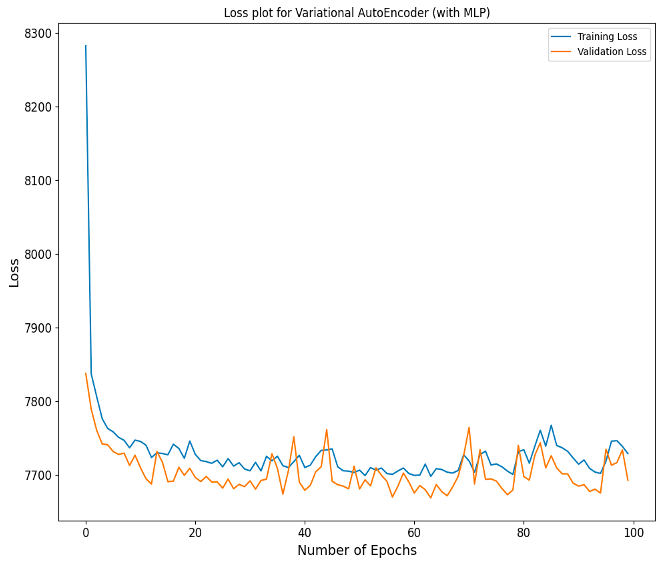
\includegraphics[width=\linewidth]{100.png}
%         \caption{Loss Curves for VAE-MLP Model trained for 100 epochs}
%         \label{fig:gen_stft}
%     \end{minipage}
%     \hfill
%     \begin{minipage}[b]{0.45\linewidth}
%         \centering
%         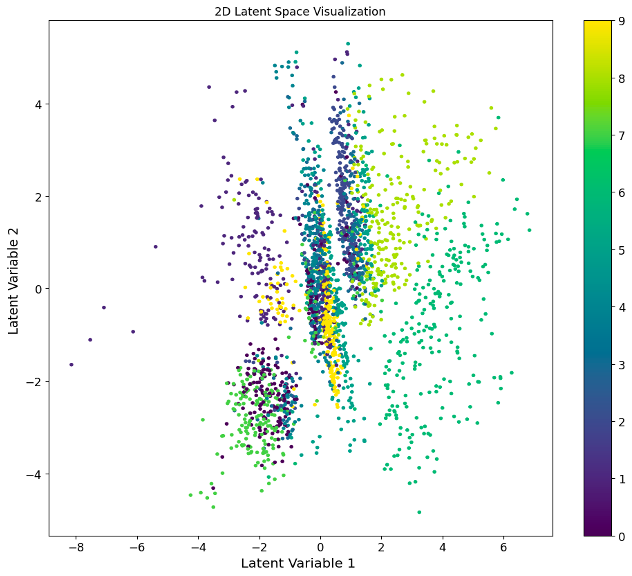
\includegraphics[width=\linewidth]{lat_100.png}
%         \caption{Latent Space Visualization on test data for VAE-MLP Model Trained for 100 epochs}
%         \label{fig:generated_audio}
%     \end{minipage}
% \end{figure}


% Despite its instability, a latent space visualization showcased improved representations compared to the earlier model. We can clearly observe in the figure above that the previously overlapping representations for digits 1 and 9 are now more distinct in comparison. The representations for other digits were observed to be distinct too in comparison however, the model seemed to fail to learn proper representation for 1 and 7, performing worse than the previous model.

% \subsubsection{Regularized VAE-MLP (100 Epochs)}
% Despite the ambiguous insights drawn from the previous model's loss plot, we adopted an intuitive approach, presuming that extended training epochs could enhance the model's performance rather than diminish it unless it was overfitting. Consequently, we opted to regularize the model and maintain the same number of training epochs. A dropout regularization rate of 30\% was implemented after each dense layer within both the encoder and decoder architectures.

% \begin{figure}[htbp]
%     \centering
%     \begin{minipage}[b]{0.45\linewidth}
%         \centering
%         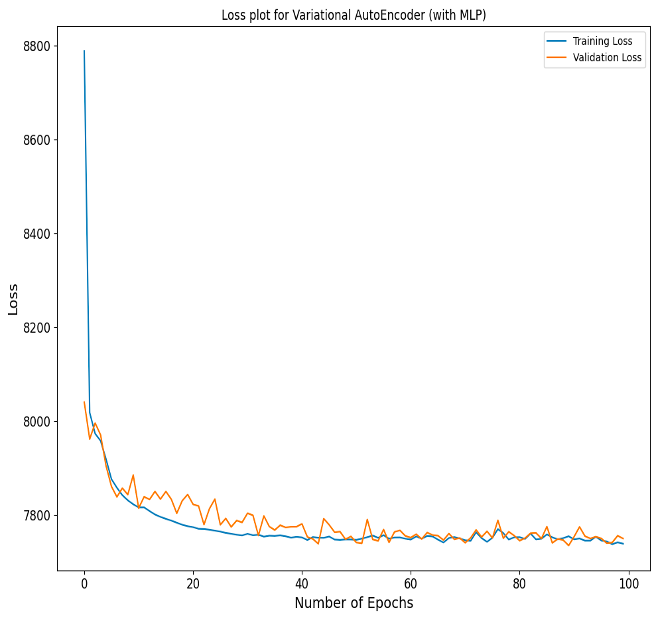
\includegraphics[width=\linewidth]{100r.png}
%         \caption{Loss Curves for regularized VAE-MLP Model trained for 100 epochs}
%         \label{fig:gen_stft}
%     \end{minipage}
%     \hfill
%     \begin{minipage}[b]{0.45\linewidth}
%         \centering
%         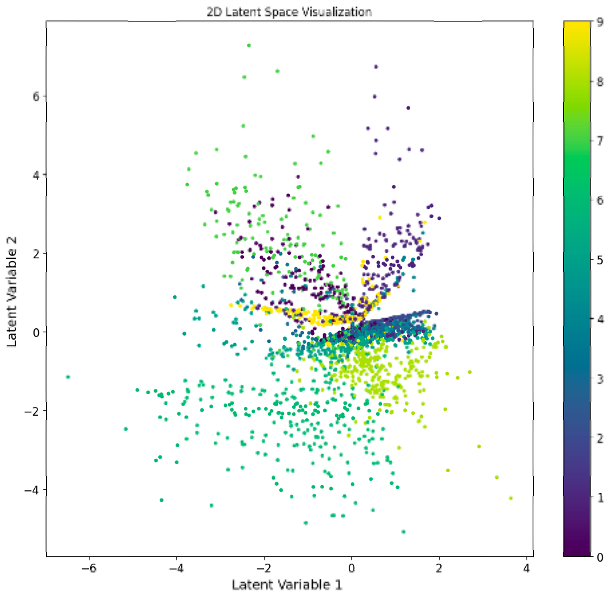
\includegraphics[width=\linewidth]{latr.png}
%         \caption{Latent Space Visualization on test data for regularized VAE-MLP Model Trained for 100 epochs}
%         \label{fig:generated_audio}
%     \end{minipage}
% \end{figure}


% Upon observing the subsequent loss plot and latent space visualization, notable findings surfaced. The model demonstrated increased stability, as indicated by both losses exhibiting a consistent downward trend, persisting until the final epoch. This indicated continual loss reduction throughout the training process. Examination of the latent space revealed more distinct and refined representations for each digit in comparison to both preceding models. Certain digits, namely 0, 5, 6, 7, 8, and 9, displayed sparser representations with reduced sample overlap. However, challenges persisted as the model encountered difficulty in learning distinct representations for digits 1, 2, 3, and 4.

% \subsection{VAE with CNN Models}

% \subsubsection{VAE-CNN (50 Epochs)}
% After employing MLP as encoding and decoding layers for VAE, we explored the use of CNN layer to do the encoding and decoding task. The architecture defined in section 3.3.2 was used to train the extracted STFT features.

% Initially, the model was trained for 50 epochs, and subsequently, the loss curves and latent space were scrutinized. The plotted loss curves indicated a consistent decrease in both training and validation losses until approximately 16 epochs. Beyond this point, the training loss continued to decrease, while the validation loss plateaued, signifying a case of overfitting. This variation, with the validation loss persisting higher than the training loss, explained that the model excelled on the training data (hence the low training loss) but struggled when generalizing to unseen data (resulting in the higher validation loss).

% \begin{figure}[htbp]
%     \centering
%     \begin{minipage}[b]{0.45\linewidth}
%         \centering
%         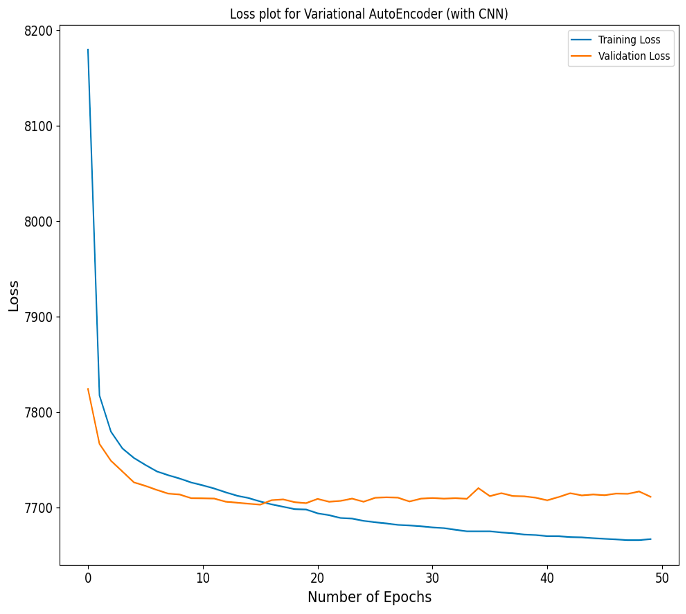
\includegraphics[width=\linewidth]{50c.png}
%         \caption{Loss Curves for VAE-CNN Model trained for 50 epochs}
%         \label{fig:gen_stft}
%     \end{minipage}
%     \hfill
%     \begin{minipage}[b]{0.45\linewidth}
%         \centering
%         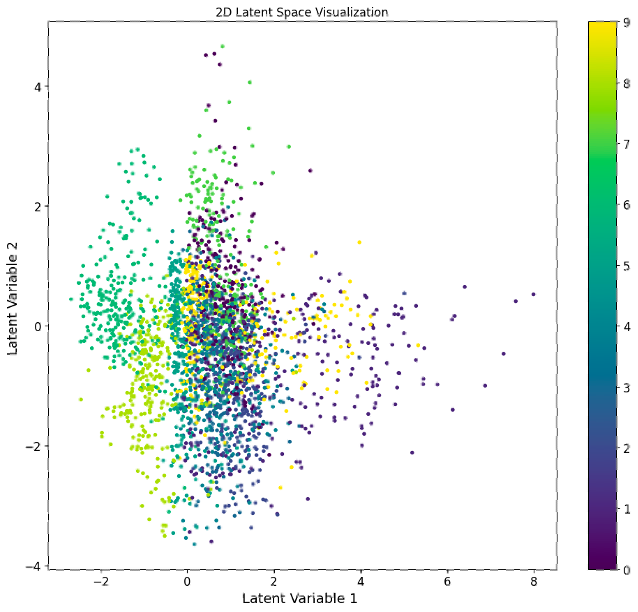
\includegraphics[width=\linewidth]{50clat.png}
%         \caption{Latent Space Visualization on test data for VAE-CNN Model Trained for 50 epochs}
%         \label{fig:generated_audio}
%     \end{minipage}
% \end{figure}


% Examining the latent space visualization provided further insights into the model's performance. The representations learned by the model appeared highly overlapped, implying an inability to distinguish unique representations for each digit. Only digits 6 and 8 exhibited somewhat distinctive representations amidst the overall lack of separation. Consequently, this model emerged as the worst-performing model among those tested.

% \subsubsection{Regularized VAE-CNN (50 Epochs)}
% As the prior VAE-CNN model exhibited clear signs of overfitting, we sought to address this issue by incorporating regularization techniques. We regularized the model using L2 regularizers (with regularization parameter (\(\lambda\)= 0.001) for the filters of the convolutional layer and 20\% dropout for the dense layers. The model was then trained on the same number of epochs (50) and the performance was observed using the loss and latent space plots.

% The loss plots showed a consistent and monotonic decline in both training and validation losses, indicating a resolution of the overfitting problem witnessed in the previous model. Notably, the decreasing loss values persisted throughout the entire training duration, suggesting continuous learning up to the final epoch.

% \begin{figure}[htbp]
%     \centering
%     \begin{minipage}[b]{0.45\linewidth}
%         \centering
%         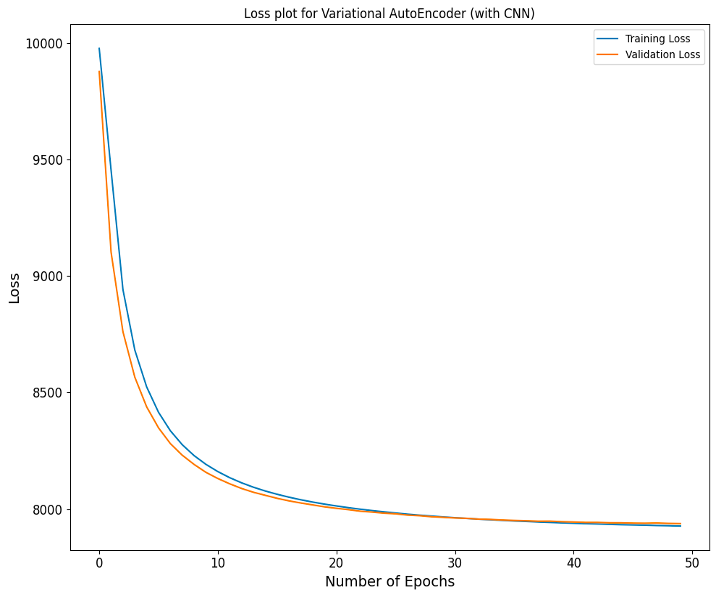
\includegraphics[width=\linewidth]{100cr.png}
%         \caption{Loss Curves for regularized VAE-CNN Model trained for 50 epochs}
%         \label{fig:gen_stft}
%     \end{minipage}
%     \hfill
%     \begin{minipage}[b]{0.45\linewidth}
%         \centering
%         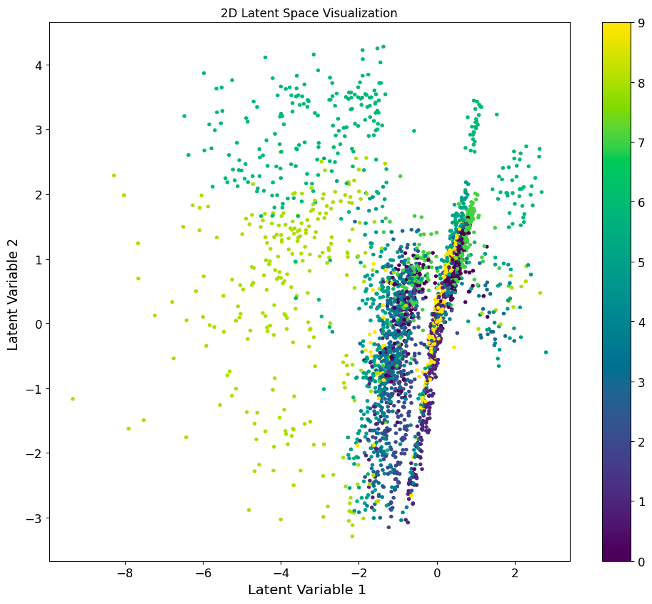
\includegraphics[width=\linewidth]{latcr.png}
%         \caption{Latent Space Visualization on test data for regularized VAE-CNN Model Trained for 50 epochs}
%         \label{fig:generated_audio}
%     \end{minipage}
% \end{figure}

% Analysis of the learned latent space exhibited enhanced performance compared to the previous VAE-CNN model, as the representations appeared more distinct. However, challenges persisted as the model struggled to effectively learn representations for all digits, demonstrating commendable performance solely for digits 4, 5, 6, 7, and 8. Despite exhibiting favorable loss curves, the model's overall improvement was marginal, ultimately underperforming compared to all VAE-MLP models evaluated.

% \begin{table}
% \centering
% \caption{Summary of the Model Outputs}
% \label{tab:my_table}
% \begin{tabular}{ l  l  l  l  l  l }

% Metrics / Models& \textbf{MLP-VAE 
% Model 1}& \textbf{MLP-VAE 
% Model 2}& \textbf{MLP-VAE 
% Regularized Model}& \textbf{CNN-VAE 
% Model 1}& \textbf{CNN-VAE 
% Regularized 
% Model}\\

% \textbf{Epochs} & 50 & 100 & 100 & 50 & 50 \\

% \textbf{Training Time
% (on Quadro k2200)}& 2.1 hrs& 5.3 hrs& 6.1 hrs& 18.7 hrs& 20.41 hrs\\

% \textbf{Training Loss} & 7673.74 & 7728.95 & 7738.79 & 7927.34 & 7987.90 \\

% \textbf{Validation Loss} & 7667.33 & 7697.56 & 7749.78 & 7937.97 & 7989.33 \\

% \textbf{Test Loss} & 7692.69 & 7707.67 & 7773.57 & 7962.82 & 7993.68 \\


% \end{tabular}

% \end{table}




\subsection{VAE with MLP Models}

\subsubsection{VAE-MLP (50 Epochs)}
During the experimentation phase, three variations of the VAE with MLP were trained and evaluated. The architecture defined in section 3.3.1 was used to train the flattened STFT features.

Initially, a basic VAE-MLP model was trained for 50 epochs, and its training and validation losses were visualized. Observing the loss plot, both the training and validation loss were decreasing and showed no signs of overfitting or underfitting.

\begin{figure}[htbp]
    \centering
    \begin{minipage}[b]{0.45\linewidth}
        \centering
        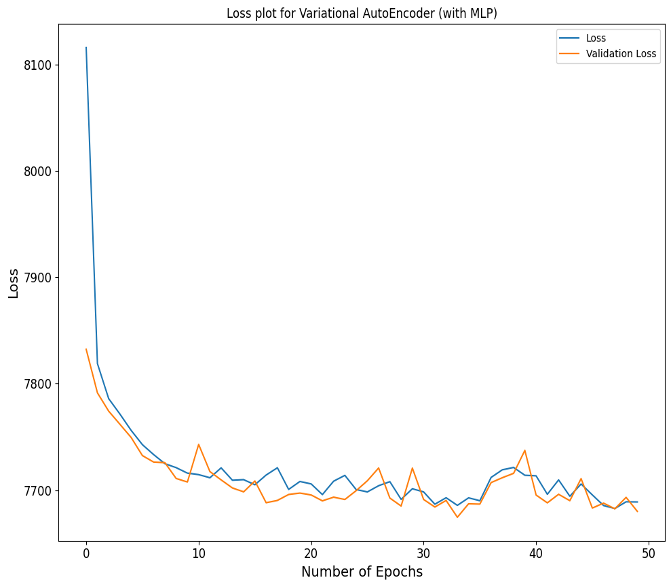
\includegraphics[width=\linewidth]{mlp_vae_50.png}
        \caption{Loss Curves for VAE-MLP Model trained for 50 epochs}
        \label{fig:gen_stft}
    \end{minipage}
    \hfill
    \begin{minipage}[b]{0.45\linewidth}
        \centering
        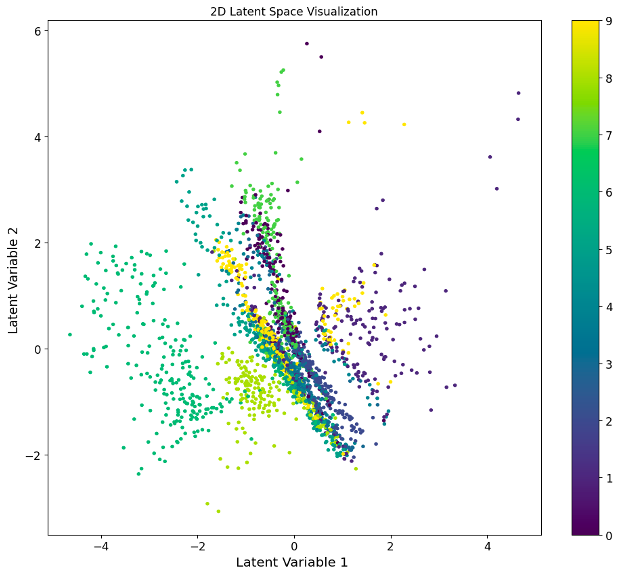
\includegraphics[width=\linewidth]{mlp_vae_lat.png}
        \caption{Latent Space Visualization on test data for VAE-MLP Model Trained for 50 epochs}
        \label{fig:generated_audio}
    \end{minipage}
\end{figure}

Since the model showed promise, we decided to observe the learned latent space representation of the model. However, the visualization clearly showed severe overlapping of the learned representations for certain digits (especially for digits 0,1,2,3, and 9), indicating the model has not learned distinctive representations for each of the digits yet. Observing the loss plot again, it was evident that while the model was learning, there remained room for additional improvement since both the losses displayed potential for further decrease (that is the losses were not observed to be saturated) in loss and learning the representations better. We therefore decided to train the model for more epochs.

\subsubsection{VAE-MLP (100 Epochs)}
The loss plot for the VAE-MLP model trained for 100 epochs showed limited improvement and instead displayed instability in the model. After approximately 70 epochs, both the training and validation losses exhibited no proper decrement. This discrepancy made it challenging to conclusively determine if the model suffered from underfitting or overfitting due to its unstable behavior.

\begin{figure}[htbp]
    \centering
    \begin{minipage}[b]{0.45\linewidth}
        \centering
        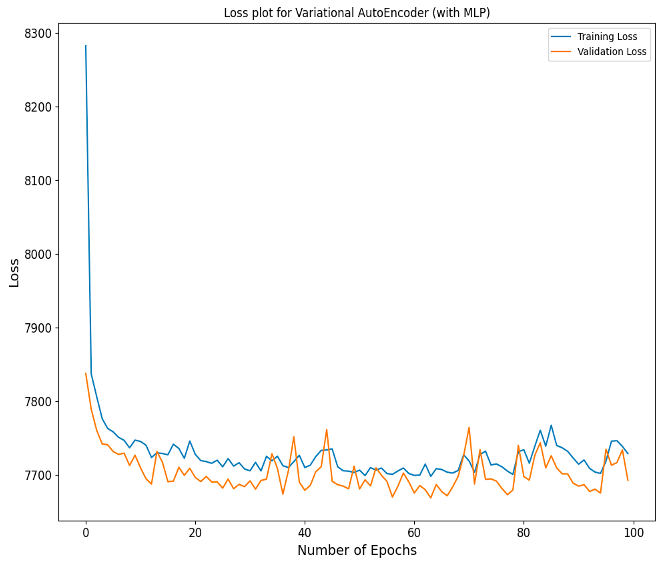
\includegraphics[width=\linewidth]{100.png}
        \caption{Loss Curves for VAE-MLP Model trained for 100 epochs}
        \label{fig:gen_stft}
    \end{minipage}
    \hfill
    \begin{minipage}[b]{0.45\linewidth}
        \centering
        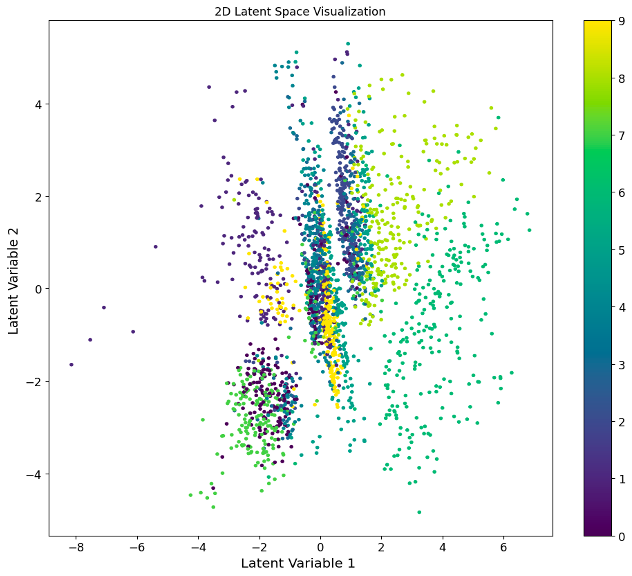
\includegraphics[width=\linewidth]{lat_100.png}
        \caption{Latent Space Visualization on test data for VAE-MLP Model Trained for 100 epochs}
        \label{fig:generated_audio}
    \end{minipage}
\end{figure}


Despite its instability, a latent space visualization showcased improved representations compared to the earlier model. We can clearly observe in the figure above that the previously overlapping representations for digits 1 and 9 are now more distinct in comparison. The representations for other digits were observed to be distinct too in comparison however, the model seemed to fail to learn proper representation for 1 and 7, performing worse than the previous model.

\subsubsection{Regularized VAE-MLP (100 Epochs)}
Despite the ambiguous insights drawn from the previous model's loss plot, we adopted an intuitive approach, presuming that extended training epochs could enhance the model's performance rather than diminish it unless it was overfitting. Consequently, we opted to regularize the model and maintain the same number of training epochs. A dropout regularization rate of 30\% was implemented after each dense layer within both the encoder and decoder architectures.

\begin{figure}[htbp]
    \centering
    \begin{minipage}[b]{0.45\linewidth}
        \centering
        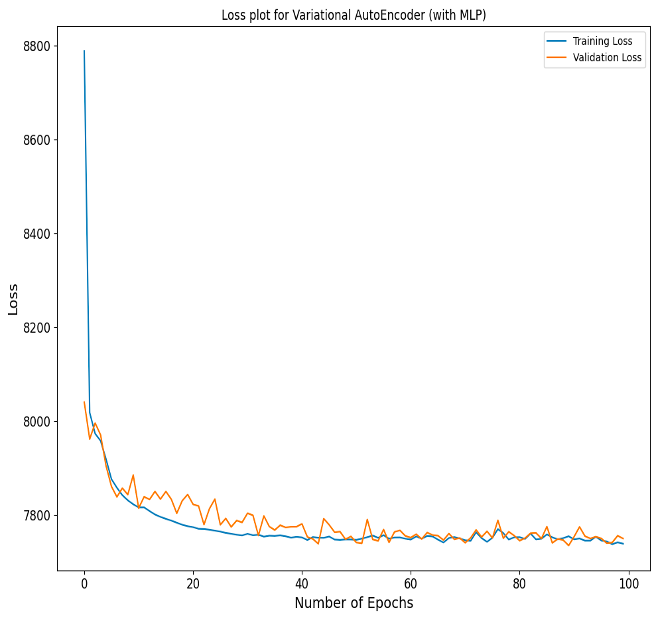
\includegraphics[width=\linewidth]{100r.png}
        \caption{Loss Curves for regularized VAE-MLP Model trained for 100 epochs}
        \label{fig:gen_stft}
    \end{minipage}
    \hfill
    \begin{minipage}[b]{0.45\linewidth}
        \centering
        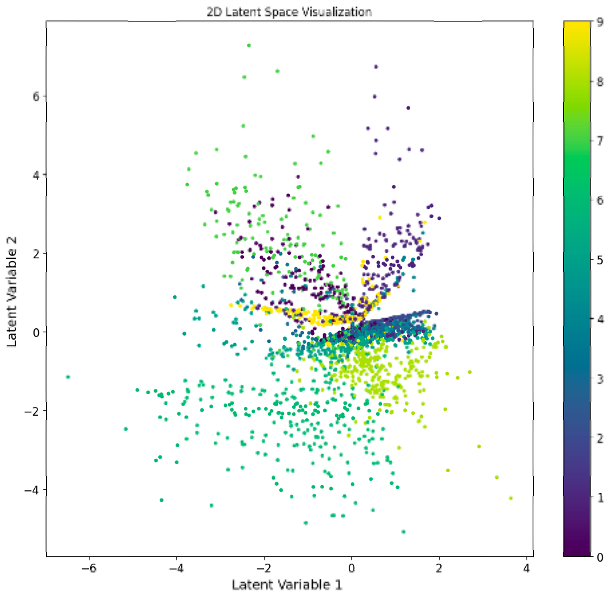
\includegraphics[width=\linewidth]{latr.png}
        \caption{Latent Space Visualization on test data for regularized VAE-MLP Model Trained for 100 epochs}
        \label{fig:generated_audio}
    \end{minipage}
\end{figure}


Upon observing the subsequent loss plot and latent space visualization, notable findings surfaced. The model demonstrated increased stability, as indicated by both losses exhibiting a consistent downward trend, persisting until the final epoch. This indicated continual loss reduction throughout the training process. Examination of the latent space revealed more distinct and refined representations for each digit in comparison to both preceding models. Certain digits, namely 0, 5, 6, 7, 8, and 9, displayed sparser representations with reduced sample overlap. However, challenges persisted as the model encountered difficulty in learning distinct representations for digits 1, 2, 3, and 4.

\subsection{VAE with CNN Models}

\subsubsection{VAE-CNN (50 Epochs)}
After employing MLP as encoding and decoding layers for VAE, we explored the use of the CNN layer to do the encoding and decoding task. The architecture defined in section 3.3.2 was used to train the extracted STFT features.

Initially, the model was trained for 50 epochs, and subsequently, the loss curves and latent space were scrutinized. The plotted loss curves indicated a consistent decrease in both training and validation losses until approximately 16 epochs. Beyond this point, the training loss continued to decrease, while the validation loss plateaued, signifying a case of overfitting. This variation, with the validation loss persisting higher than the training loss, explained that the model excelled on the training data (hence the low training loss) but struggled when generalizing to unseen data (resulting in the higher validation loss).

\begin{figure}[htbp]
    \centering
    \begin{minipage}[b]{0.45\linewidth}
        \centering
        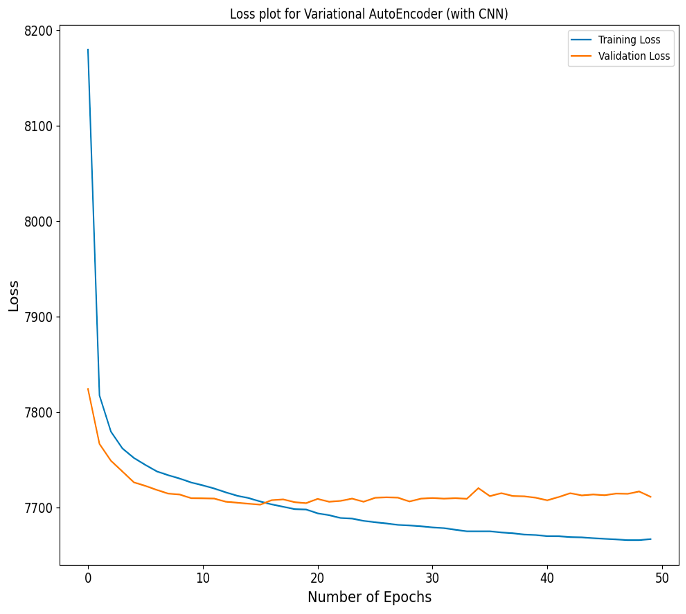
\includegraphics[width=\linewidth]{50c.png}
        \caption{Loss Curves for VAE-CNN Model trained for 50 epochs}
        \label{fig:gen_stft}
    \end{minipage}
    \hfill
    \begin{minipage}[b]{0.45\linewidth}
        \centering
        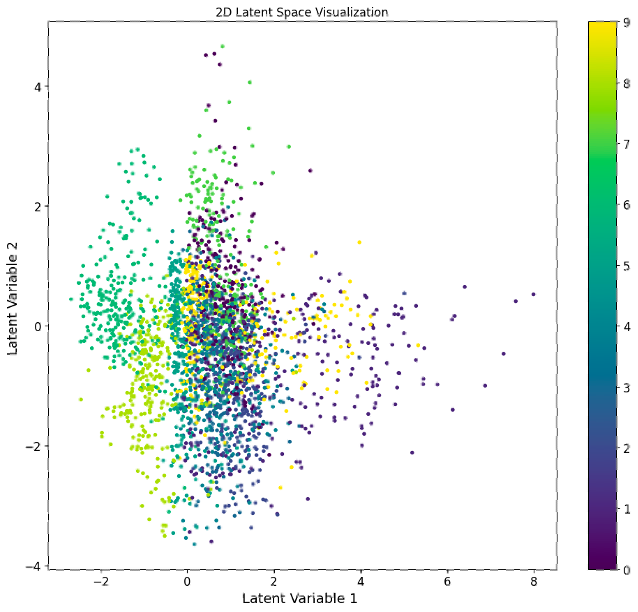
\includegraphics[width=\linewidth]{50clat.png}
        \caption{Latent Space Visualization on test data for VAE-CNN Model Trained for 50 epochs}
        \label{fig:generated_audio}
    \end{minipage}
\end{figure}


Examining the latent space visualization provided further insights into the model's performance. The representations learned by the model appeared highly overlapped, implying an inability to distinguish unique representations for each digit. Only digits 6 and 8 exhibited somewhat distinctive representations amidst the overall lack of separation. Consequently, this model emerged as the worst-performing model among those tested.

\subsubsection{Regularized VAE-CNN (50 Epochs)}
As the prior VAE-CNN model exhibited clear signs of overfitting, we sought to address this issue by incorporating regularization techniques. We regularized the model using L2 regularizers (with regularization parameter (\(\lambda\)= 0.001) for the filters of the convolutional layer and 20\% dropout for the dense layers. The model was then trained on the same number of epochs (50) and the performance was observed using the loss and latent space plots.

The loss plots showed a consistent and monotonic decline in both training and validation losses, indicating a resolution of the overfitting problem witnessed in the previous model. Notably, the decreasing loss values persisted throughout the entire training duration, suggesting continuous learning up to the final epoch.

\begin{figure}[htbp]
    \centering
    \begin{minipage}[b]{0.45\linewidth}
        \centering
        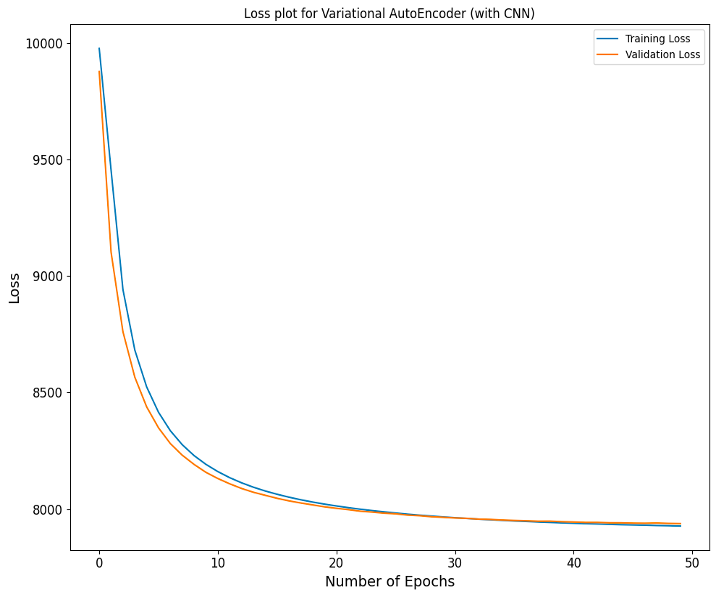
\includegraphics[width=\linewidth]{100cr.png}
        \caption{Loss Curves for regularized VAE-CNN Model trained for 50 epochs}
        \label{fig:gen_stft}
    \end{minipage}
    \hfill
    \begin{minipage}[b]{0.45\linewidth}
        \centering
        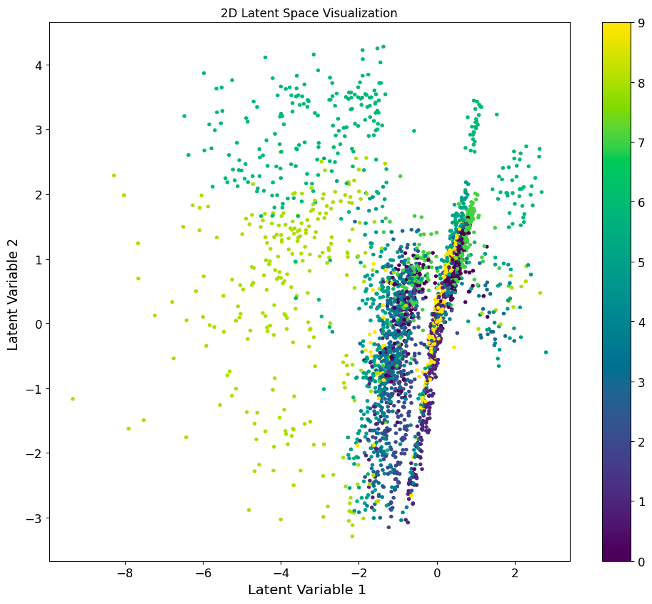
\includegraphics[width=\linewidth]{latcr.png}
        \caption{Latent Space Visualization on test data for regularized VAE-CNN Model Trained for 50 epochs}
        \label{fig:generated_audio}
    \end{minipage}
\end{figure}

Analysis of the learned latent space exhibited enhanced performance compared to the previous VAE-CNN model, as the representations appeared more distinct. However, challenges persisted as the model struggled to effectively learn representations for all digits, demonstrating commendable performance solely for digits 4, 5, 6, 7, and 8. Despite exhibiting favorable loss curves, the model's overall improvement was marginal, ultimately underperforming compared to all VAE-MLP models evaluated.

% \begin{table}
% \centering
% \caption{Summary of the Model Outputs}
% \label{tab:my_table}
% \begin{tabular}{l l l l l l}

% \textbf{Metrics / Models}& \textbf{MLP-VAE Model 1}& \textbf{MLP-VAE 
% Model 2}& \textbf{MLP-VAE 
% Regularized Model}& \textbf{CNN-VAE 
% Model 1}& \textbf{CNN-VAE 
% Regularized 
% Model}\\

% \textbf{Epochs} & 50 & 100 & 100 & 50 & 50 \\

% \textbf{Training Time (on Quadro k2200)}& 2.1 hrs& 5.3 hrs& 6.1 hrs& 18.7 hrs& 20.41 hrs\\

% \textbf{Training Loss} & 7673.74 & 7728.95 & 7738.79 & 7927.34 & 7987.90 \\

% \textbf{Validation Loss} & 7667.33 & 7697.56 & 7749.78 & 7937.97 & 7989.33 \\

% \textbf{Test Loss} & 7692.69 & 7707.67 & 7773.57 & 7962.82 & 7993.68 \\


% \end{tabular}

% \end{table}

% \usepackage{graphicx}


\begin{table}[!h]
\caption{Summary of the Model Outputs}
\centering
\begin{tabular}{l|lllll}
\textbf{Metrics/Models} &
  \textbf{\begin{tabular}[c]{@{}l@{}}MLP-VAE\\ Model 1\end{tabular}} &
  \textbf{\begin{tabular}[c]{@{}l@{}}MLP-VAE\\ Model 1\end{tabular}} &
  \textbf{\begin{tabular}[c]{@{}l@{}}MLP-VAE\\ Regularized \\ Model\end{tabular}} &
  \textbf{\begin{tabular}[c]{@{}l@{}}CNN-VAE\\ Model 1\end{tabular}} &
  \textbf{\begin{tabular}[c]{@{}l@{}}CNN-VAE\\ Regularized\\ Model\end{tabular}} \\ \hline
\textbf{Epochs}                                                                 & 50      & 100     & 100     & 50       & 50        \\
\textbf{\begin{tabular}[c]{@{}l@{}}Training Time\\ (Quadro k2200)\end{tabular}} & 2.1 hrs & 5.3 hrs & 6.1 hrs & 18.7 hrs & 20.41 hrs \\
\textbf{Training Loss}                                                          & 7673.74 & 7728.95 & 7738.79 & 7927.34  & 7987.90   \\
\textbf{Validation Loss}                                                        & 7667.33 & 7697.56 & 7749.78 & 7937.97  & 7989.33   \\
\textbf{Test Loss}                                                              & 7692.69 & 7707.67 & 7773.57 & 7962.82  & 7993.68  
\end{tabular}
\end{table}



\begin{figure}[htbp]
    \centering
    \begin{subfigure}[b]{0.45\linewidth}
        \centering
        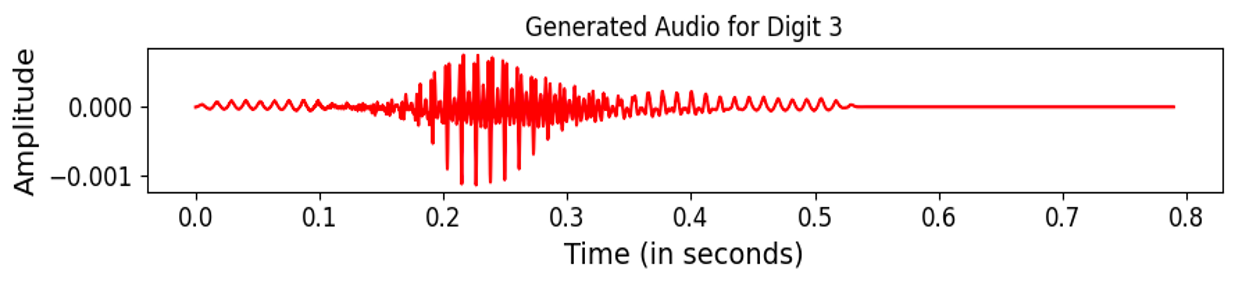
\includegraphics[width=\linewidth]{abc11.png}
        % \caption{Enter Caption 1}
        \label{fig:sub1}
    \end{subfigure}
    \hfill
    \begin{subfigure}[b]{0.45\linewidth}
        \centering
        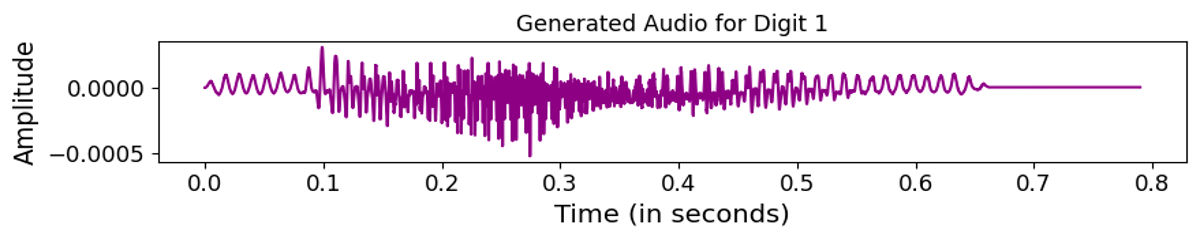
\includegraphics[width=\linewidth]{gen_1.png}
        % \caption{Enter Caption 2}
        \label{fig:sub2}
    \end{subfigure}
    
    \medskip
    
    \begin{subfigure}[b]{0.45\linewidth}
        \centering
        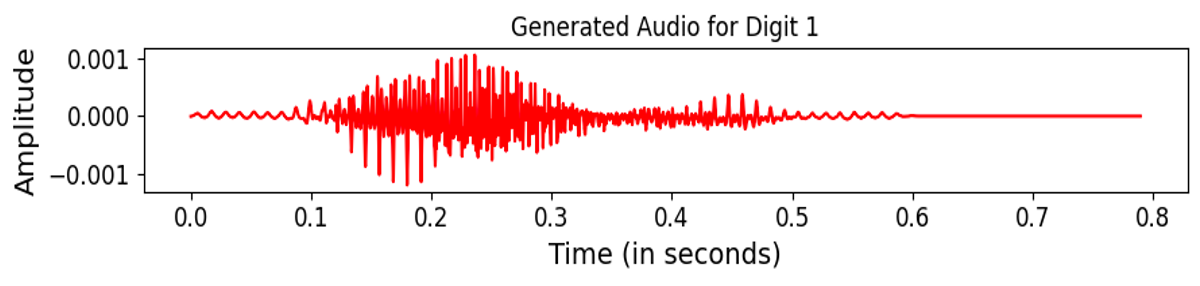
\includegraphics[width=\linewidth]{ab2.png}
        % \caption{Enter Caption 3}
        \label{fig:sub3}
    \end{subfigure}
    \hfill
    \begin{subfigure}[b]{0.45\linewidth}
        \centering
        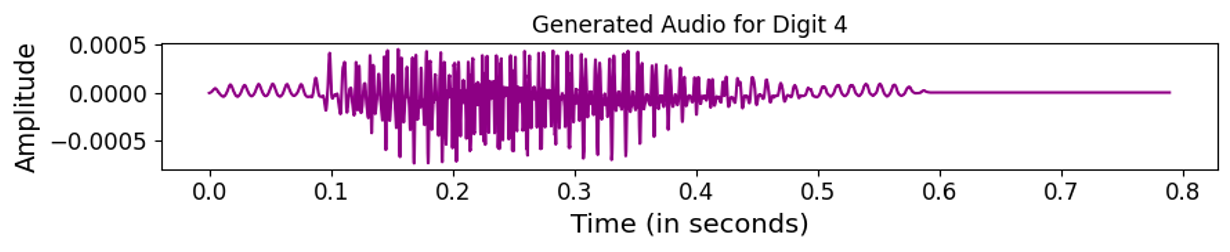
\includegraphics[width=\linewidth]{gen_4.png}
        % \caption{Enter Caption 4}
        \label{fig:sub4}
    \end{subfigure}
    
    \bigskip
    
    \begin{subfigure}[b]{0.45\linewidth}
        \centering
        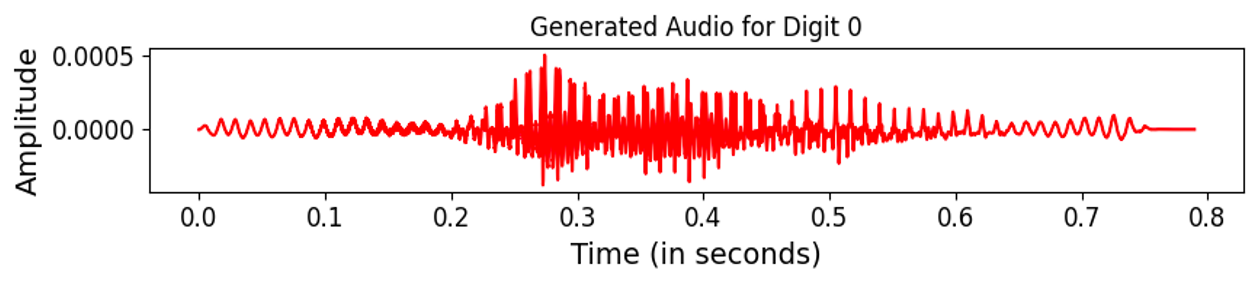
\includegraphics[width=\linewidth]{abc3.png}
        % \caption{Enter Caption 5}
        \label{fig:sub5}
    \end{subfigure}
    \hfill
    \begin{subfigure}[b]{0.45\linewidth}
        \centering
        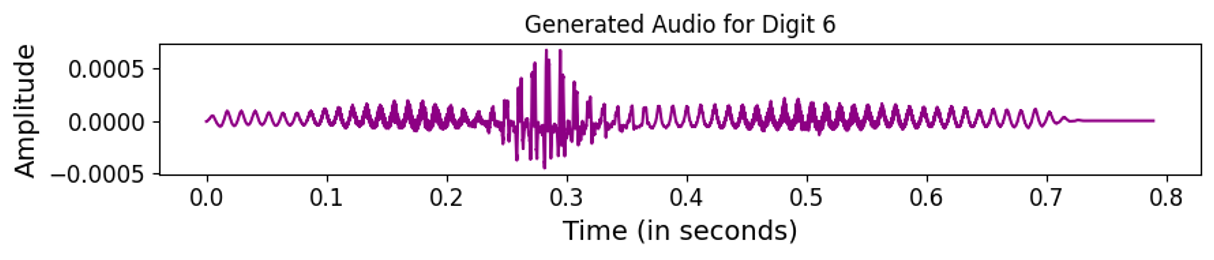
\includegraphics[width=\linewidth]{gen6.png}
        % \caption{Enter Caption 6}
        \label{fig:sub6}
    \end{subfigure}
    
    \medskip
    
    \begin{subfigure}[b]{0.45\linewidth}
        \centering
        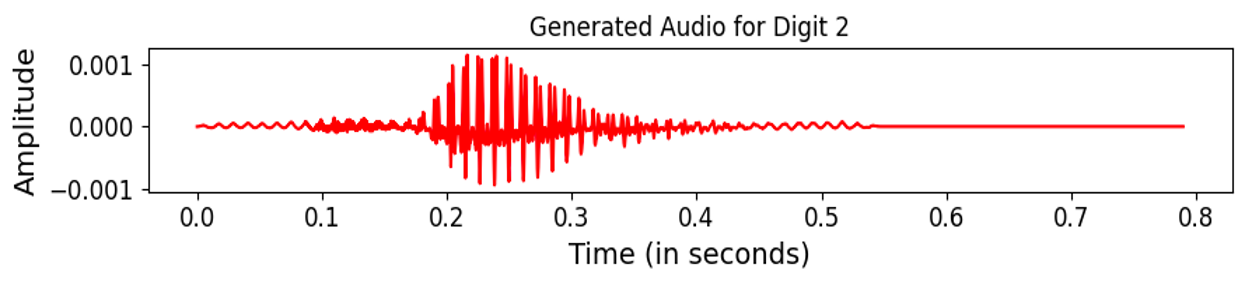
\includegraphics[width=\linewidth]{abc4.png}
        \caption{Generated Audio from VAE-MLP Model}
        \label{fig:sub7}
    \end{subfigure}
    \hfill
    \begin{subfigure}[b]{0.45\linewidth}
        \centering
        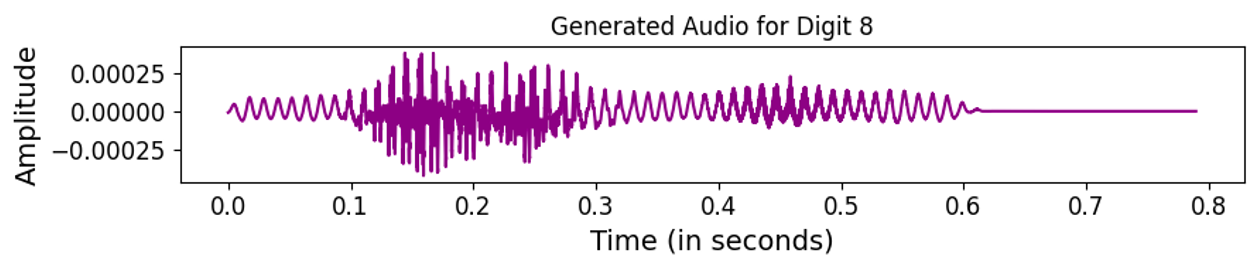
\includegraphics[width=\linewidth]{gen8.png}
        \caption{Generated Audio from VAE-CNN Model}
        \label{fig:sub8}
    \end{subfigure}
    
    \caption{Final Synthesized Audio by the Generative Models}
    \label{fig:main_figure}
\end{figure}


\section{Discussion and Future Work}
\subsection{Discussion}
In our study, we explored various strategies to enhance the performance of variational autoencoders (VAEs) in the context of speech synthesis using the Audio-MNIST dataset. Out of the five VAE variants trained, the regularized VAE with MLP, trained for 100 epochs, exhibited the most promising performance for the generation task. This model showcased the most distinctive latent representations for spoken digits among the tested variants.

Furthermore, our findings suggest several key considerations for improving VAE performance.

\begin{itemize}
    \item \textbf{Increasing Latent Space Dimension: }One possible approach to potentially enhance the model's performance is by expanding the dimensionality of the latent space. This expansion might allow for a more intricate and nuanced representation of the input data, potentially capturing more intricate features.
    \item \textbf{Optimization and Model Refinement: }Fine-tuning the model's hyperparameters, such as the regularization parameters, could lead to improved performance. Exploring different configurations and conducting systematic parameter tuning may further optimize the model's ability to generate high-quality speech samples.
    \item \textbf{\textbf{Data Augmentation and Model Scaling: }}Increasing the size and diversity of the training dataset could contribute to better model generalization and performance. Augmenting the dataset with additional varied samples might enhance the model's ability to capture a wider range of speech variations.
\end{itemize}

\subsection{Future Directions}
\begin{itemize}
    \item Extending this study to datasets containing full sentences or more complex linguistic structures beyond individual digits could be a valuable future direction. 
    \item By applying VAEs to larger and more diverse speech datasets, we could explore their potential to generate more extended and coherent speech sequences.
\end{itemize}

\section{Conclusion}
This project highlights the potential of variational autoencoders (VAEs) in speech synthesis tasks, specifically in generating spoken digits. By leveraging VAEs, we aimed to achieve higher fidelity and distinctiveness in generating spoken digit sequences. Further exploration and optimization of VAE architectures and training strategies could lead to more advanced applications in speech synthesis and related domains.



\bibliographystyle{ieeetr}
\bibliography{ref}

\section{APPENDIX}
\appendix
\section{Code}
Code and generated audio samples is available at: https://github.com/Bot-Ro-Bot/Exploring-Gen-AI-for-Audio-Synthesis 

\section{Tech Stack}
\begin{multicols}{4} % Set the number of columns (adjust as needed)
\raggedright % Align the items to the left
\begin{itemize}
    \item Keras
    \item Tensorflow
    \item Pickle
    \item Glob
    \item Librosa
    \item Tqdm
    \item Pandas
    \item Numpy
    \item SciPy
    \item Math
    \item Sklearn
    \item Matplotlib
    \item IPython
\end{itemize}
\end{multicols}

\section{Color Code}
\begin{table}[h]
    \centering
    \caption{Color Code for Plots}
    \label{tab:my_label}
    \begin{tabular}{|c|c|}
        \hline
        \rowcolor{blue!20} \textcolor{blue}{Blue} & Raw and unmanipulated data \\
        \hline
        \rowcolor{red!20} \textcolor{red}{Red} & Processed Data \\
        \hline
        \rowcolor{purple!20} \textcolor{purple}{Purple} & Generated Data \\
        \hline
    \end{tabular}
\end{table}


\section{Additional Plots}
\begin{figure}[h!]
    \centering
    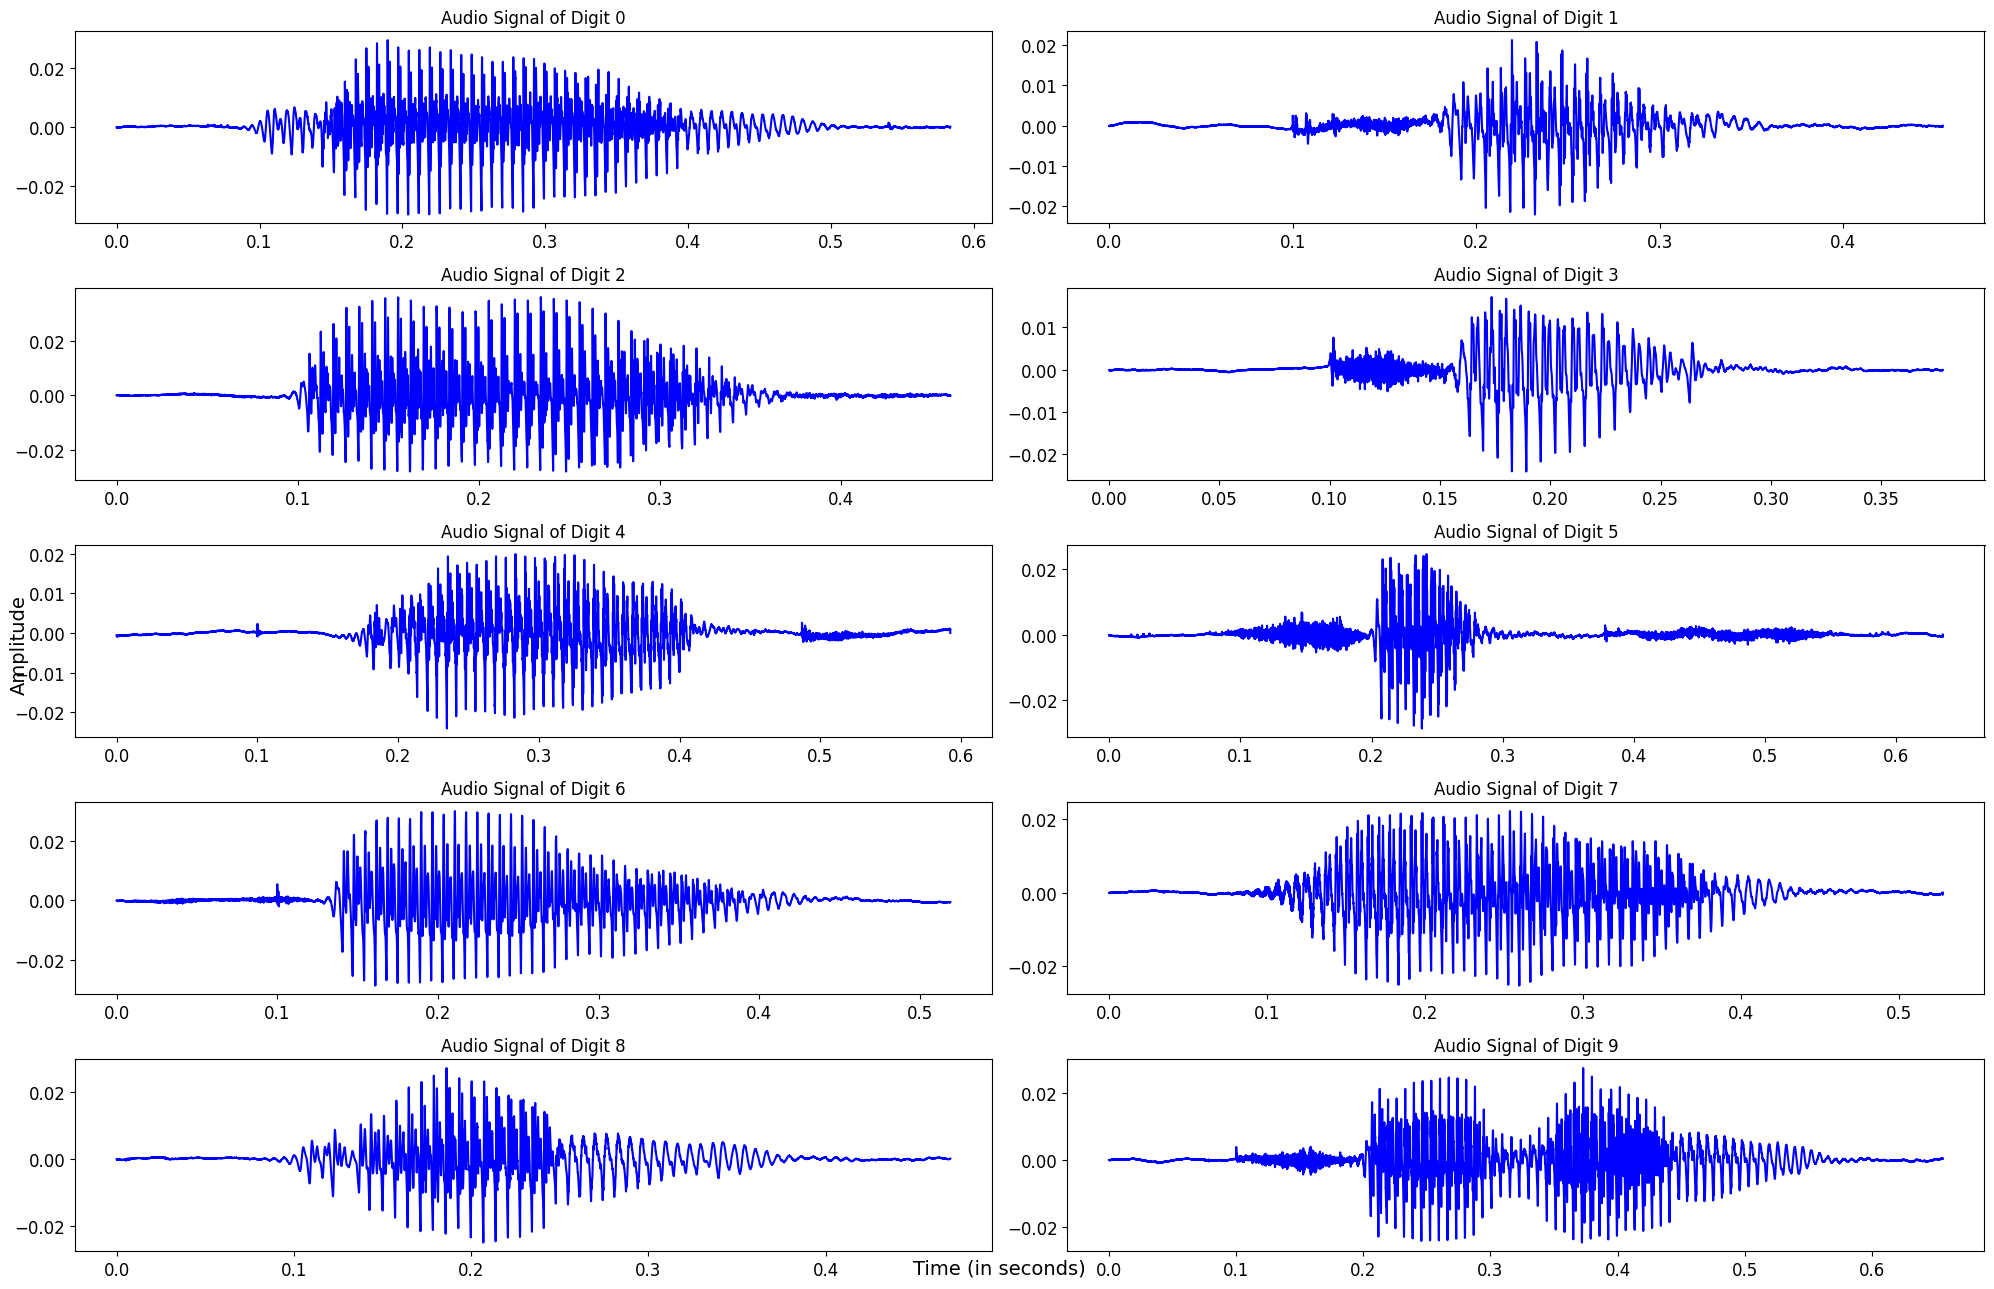
\includegraphics[width=0.9\linewidth]{figures/raw_all.png}
    \caption{Audio Signals for All Digits}
    \label{fig:enter-label}
\end{figure}


\begin{figure}[h!]
    \centering
    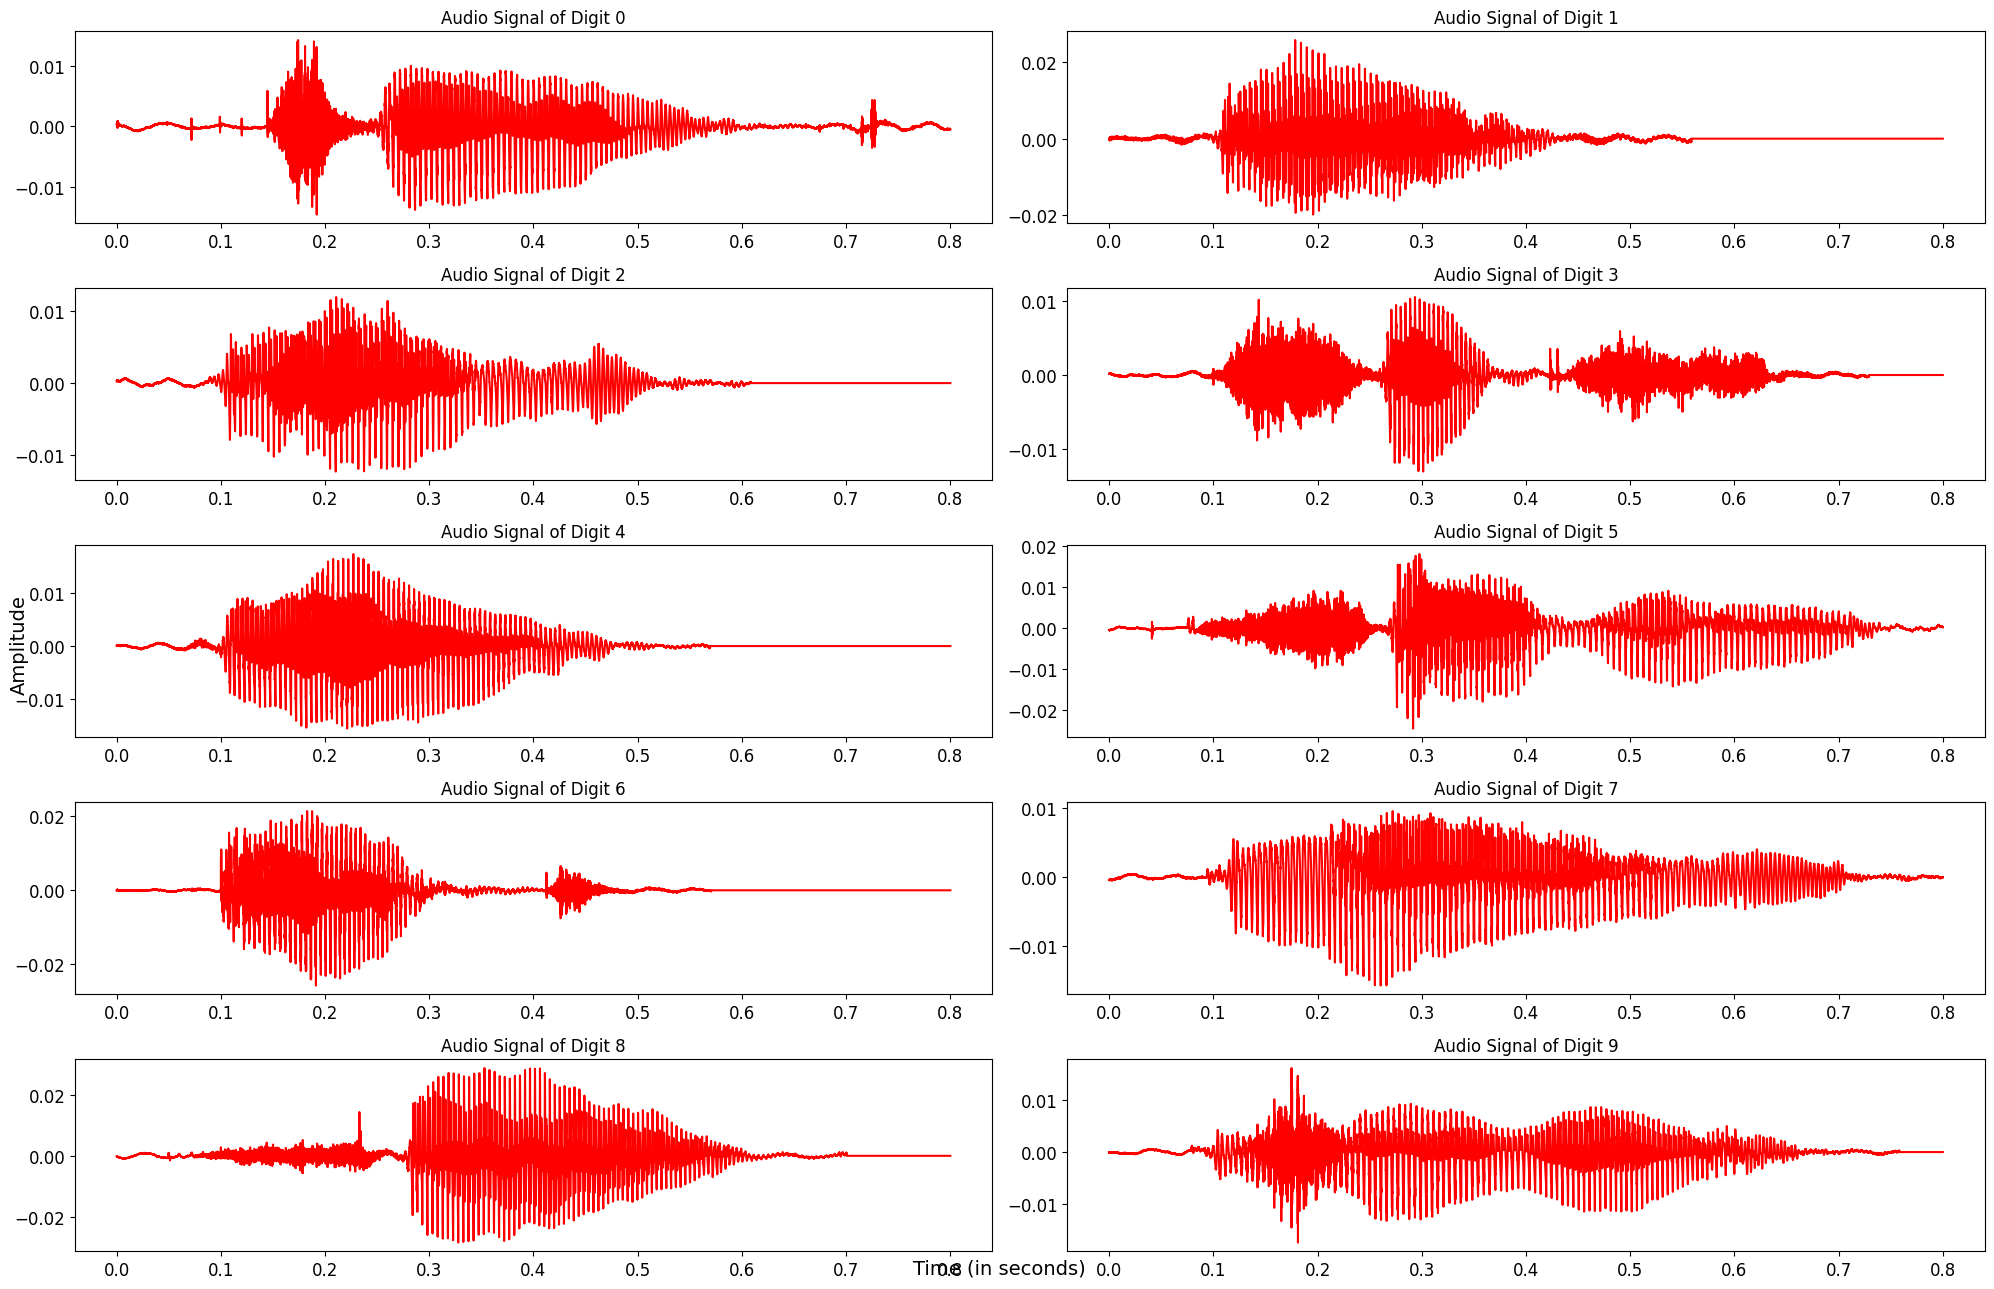
\includegraphics[width=0.9\linewidth]{figures/raw_normal.png}
    \caption{Normalized Audio Signals for All Digits}
    \label{fig:enter-label}
\end{figure}

\begin{figure}[h!]
    \centering
    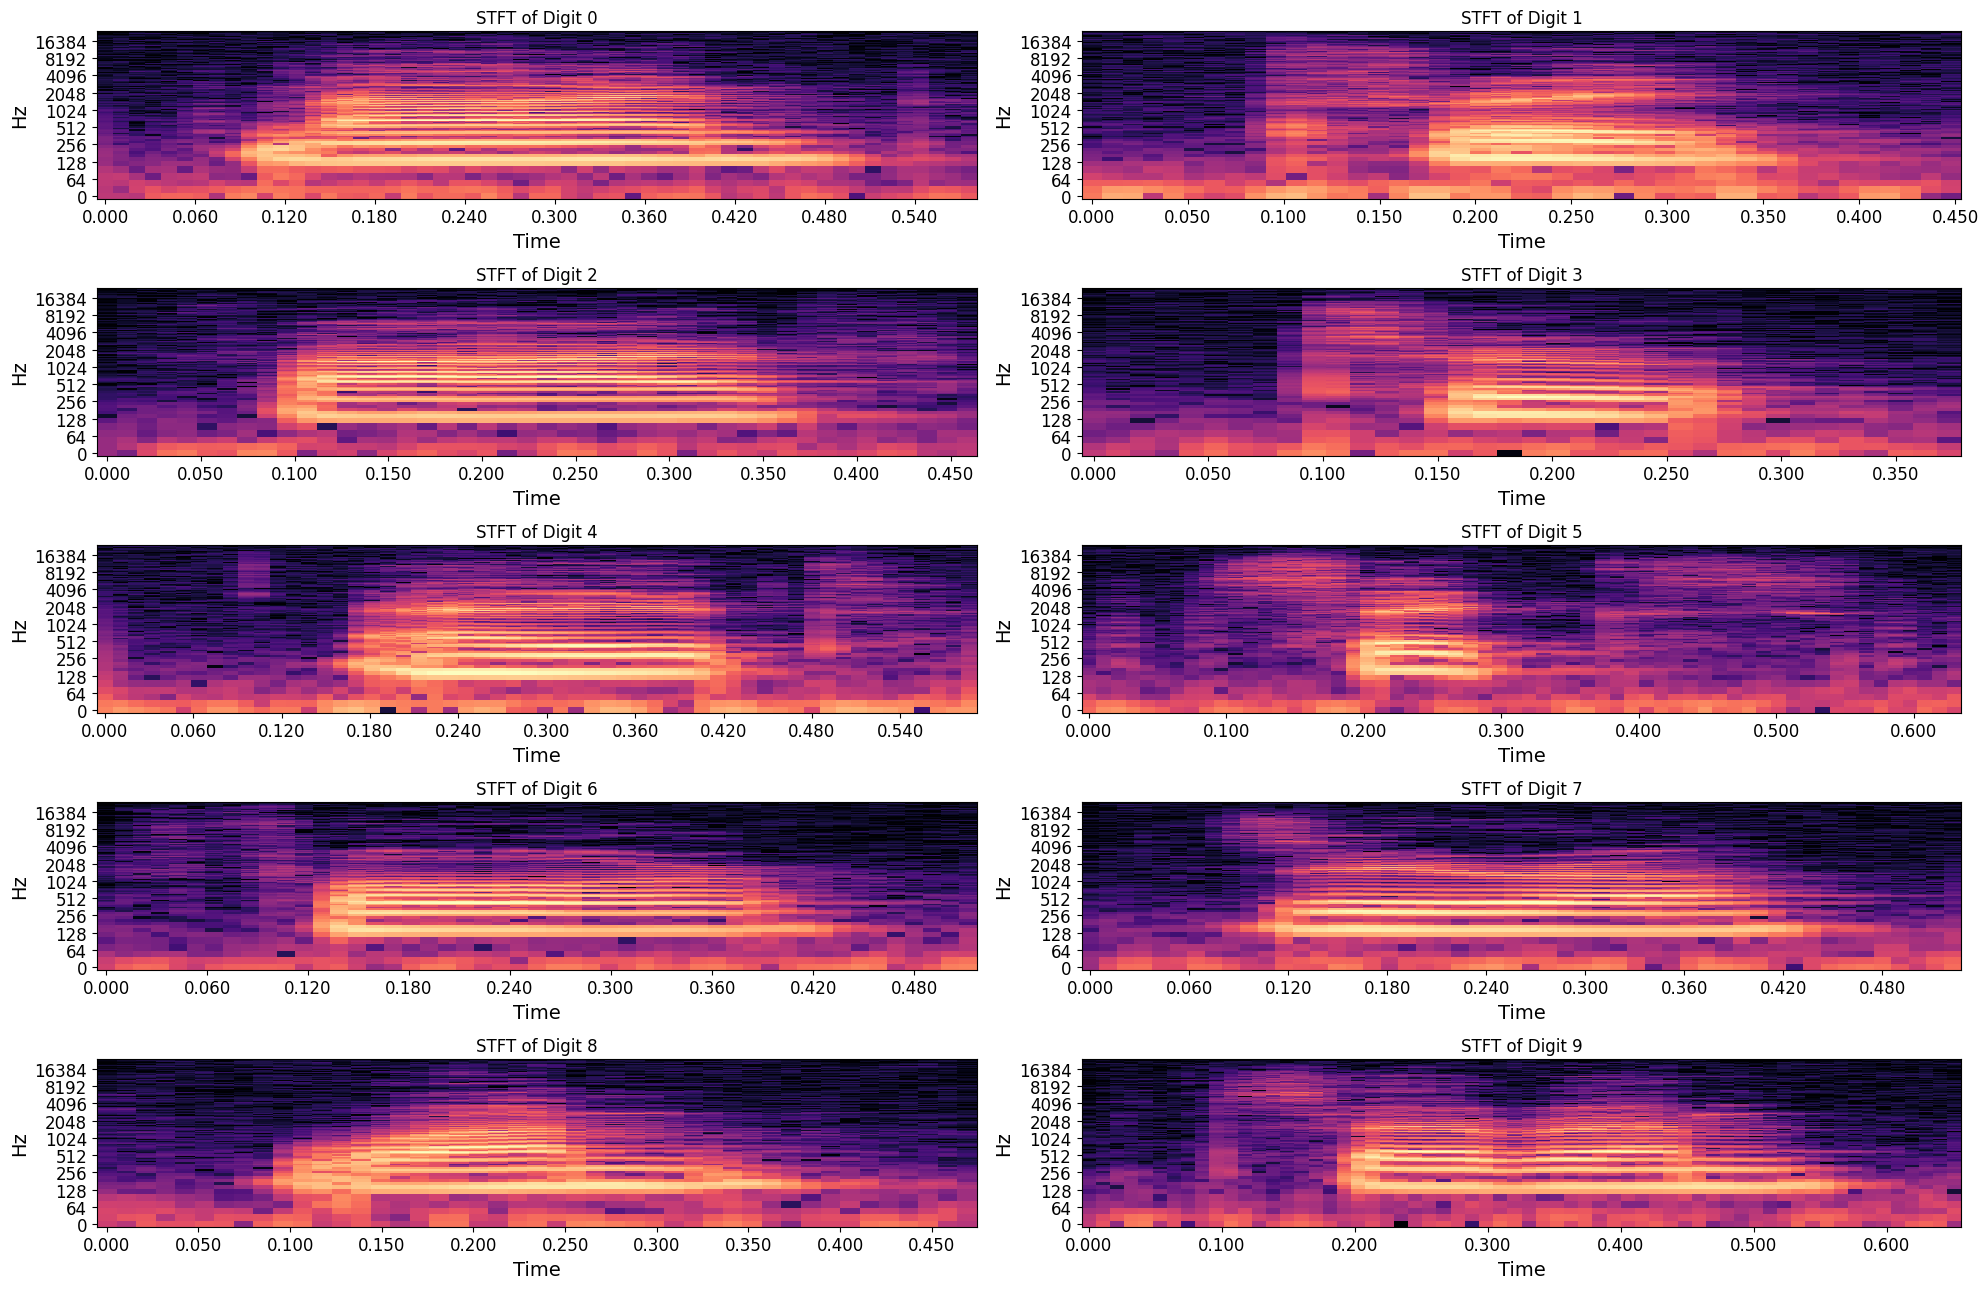
\includegraphics[width=0.9\linewidth]{figures/spectrogram_all.png}
    \caption{STFT of All Digits}
    \label{fig:enter-label}
\end{figure}


\begin{figure}[htbp]
    \centering
    \begin{subfigure}[b]{0.45\linewidth}
        \centering
        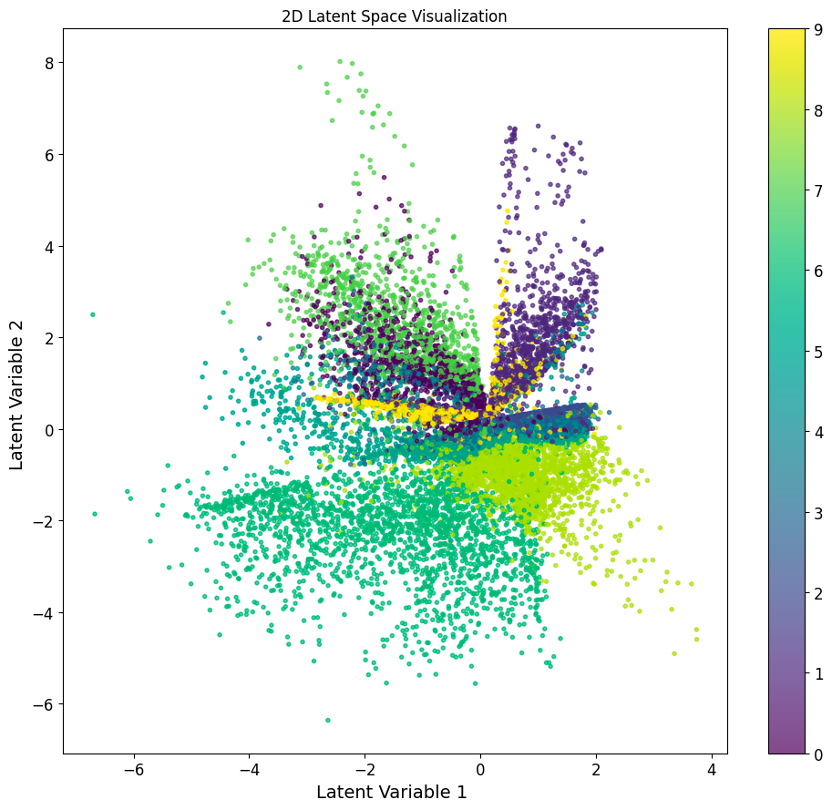
\includegraphics[width=\linewidth]{mlp100r_train.png}
        \caption{Latent Space for regularized VAE-MLP Model 100 epochs on Training Data}
        \label{fig:sub1}
    \end{subfigure}
    \hfill
    \begin{subfigure}[b]{0.45\linewidth}
        \centering
        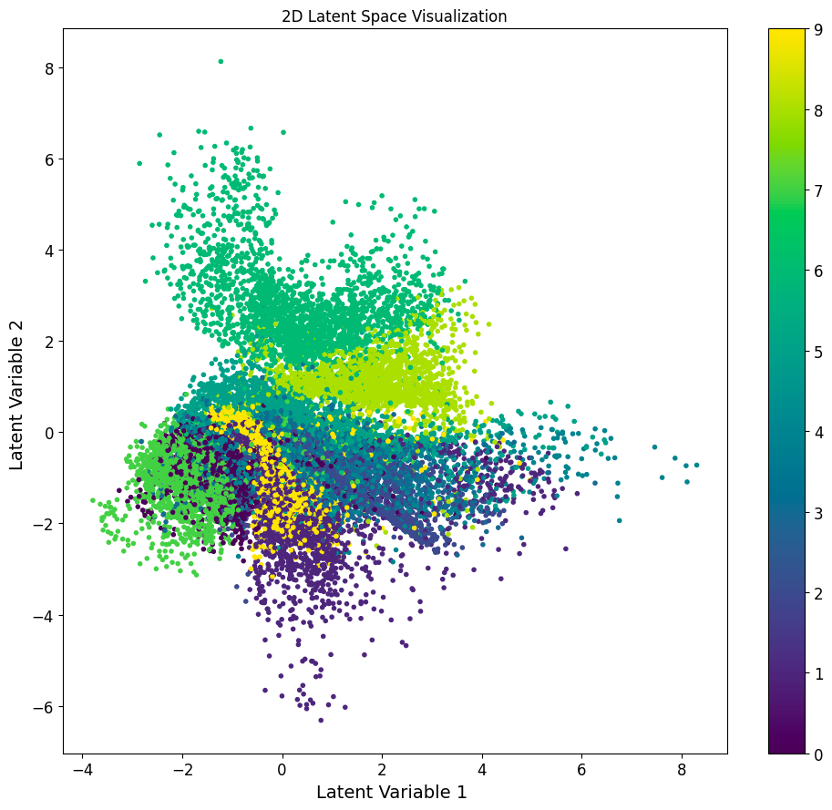
\includegraphics[width=\linewidth]{abc.png}
        \caption{Latent Space for Training Data on VAE-MLP Model 50 epochs}
        \label{fig:sub2}
    \end{subfigure}
    \caption{Comparison of Latent Spaces}
    \label{fig:main_figure}
\end{figure}


% \begin{figure}[htbp]
%     \centering
%     \begin{subfigure}[b]{0.5\linewidth}
%         \centering
%         \includegraphics[width=\linewidth]{gen_1.png}
%         \caption{Enter Caption 1}
%         \label{fig:sub1}
%     \end{subfigure}
%     \hfill
%     \begin{subfigure}[b]{0.5\linewidth}
%         \centering
%         \includegraphics[width=\linewidth]{gen_4.png}
%         \caption{Enter Caption 2}
%         \label{fig:sub2}
%     \end{subfigure}
    
%     \medskip
    
%     \begin{subfigure}[b]{0.5\linewidth}
%         \centering
%         \includegraphics[width=\linewidth]{gen6.png}
%         \caption{Enter Caption 3}
%         \label{fig:sub3}
%     \end{subfigure}
%     \hfill
%     \begin{subfigure}[b]{0.5\linewidth}
%         \centering
%         \includegraphics[width=\linewidth]{gen8.png}
%         \caption{Enter Caption 4}
%         \label{fig:sub4}
%     \end{subfigure}
    
%     \caption{Arrangement of Figures in 2x2 Setting}
%     \label{fig:main_figure}
% \end{figure}



% \begin{figure}
%     \centering
%     \includegraphics[width=0.5\linewidth]{abc11.png}
%     \caption{Enter Caption}
%     \label{fig:enter-label}
% \end{figure}

% \begin{figure}
%     \centering
%     \includegraphics[width=0.5\linewidth]{ab2.png}
%     \caption{Enter Caption}
%     \label{fig:enter-label}
% \end{figure}

% \begin{figure}
%     \centering
%     \includegraphics[width=0.5\linewidth]{abc3.png}
%     \caption{Enter Caption}
%     \label{fig:enter-label}
% \end{figure}

% \begin{figure}
%     \centering
%     \includegraphics[width=0.5\linewidth]{abc4.png}
%     \caption{Enter Caption}
%     \label{fig:enter-label}
% \end{figure}

% \begin{figure}
%     \centering
%     \includegraphics[width=0.5\linewidth]{gen_1.png}
%     \caption{Enter Caption}
%     \label{fig:enter-label}
% \end{figure}

% \begin{figure}
%     \centering
%     \includegraphics[width=0.5\linewidth]{gen_4.png}
%     \caption{Enter Caption}
%     \label{fig:enter-label}
% \end{figure}

% \begin{figure}
%     \centering
%     \includegraphics[width=0.5\linewidth]{gen6.png}
%     \caption{Enter Caption}
%     \label{fig:enter-label}
% \end{figure}

% \begin{figure}
%     \centering
%     \includegraphics[width=0.5\linewidth]{gen8.png}
%     \caption{Enter Caption}
%     \label{fig:enter-label}
% \end{figure}






\end{document}
